\documentclass[]{article}
\usepackage{amsmath}
\usepackage{amsfonts}
\usepackage{amssymb}
\usepackage{hyperref}
\usepackage{gensymb}
\usepackage{graphicx}
\usepackage{svg}
\usepackage{bbding}
\usepackage{mathtools}
\usepackage{centernot} % not parallel, etc.
\usepackage{lmodern}
\usepackage{morewrites}
\usepackage{xcolor,sectsty} % colorful sections
\usepackage[left=10mm, top=10mm, right=10mm, bottom=10mm, nohead, nofoot]{geometry} %Exam
%\usepackage{bigints}
\usepackage{dsfont} %mathbb 1
\usepackage{esint} % beatiful integrals


\DeclareFontFamily{OMX}{lmex}{}
\DeclareFontShape{OMX}{lmex}{m}{n}{<-> lmex10}{}


%colors of sections
\definecolor{secfont}{RGB}{46,116,181}
\definecolor{subfont}{RGB}{146,23,57}
\definecolor{parfont}{RGB}{19,127,43}
\definecolor{subparfont}{RGB}{7,11,100}

\subsectionfont{\color{subfont}}
\sectionfont{\color{secfont}}
\paragraphfont{\color{parfont}}
\subparagraphfont{\color{subparfont}}

%\usepackage{babel}[english]
%opening
\title{104222 - Probability Theory}
\author{Ross Pinsky}

\parindent=0em
\begin{document}


\maketitle

\begin{abstract}

\end{abstract}

\tableofcontents
\section{Intro}
\subsection{Probabilistic experiments}
\begin{enumerate}
	\item Throwing two dices. Possible results: $\left\{(i,j) : 1\leq 1,6 \leq 6 \right\}$.
	$$P(\left\{ (i,j) \right\}) = \frac{1}{36}$$
	\item Throwing of coin until we get heads (H). $\left\{ 1,2,3,\dots \right\}$. Probability is $$P(\left\{ n \right\})\left(\frac{1}{2}\right)^n$$
	\item Choosing a random number in $[0,2]$. Random means that $$P\bigg( (a,b) \bigg) = \frac{b-a}{2}$$
\end{enumerate}

\paragraph{State space} is a space of all possible results of the experiment. Is denoted with $\Omega$.
\paragraph{Event} $A$ is subset of state space. $A \subset \Omega$.
\paragraph{Function of probability} (or measure of probability) is a function defined on particular set of events in $\Omega$ and has following properties:
\begin{enumerate}
	\item $P(\emptyset) = 0$ and $P(\Omega) = 1$.
	\item $0\leq P(A) \leq 1$ if $P(A)$ is defined.
	\item Sigma-additivity: if $\left\{ A_n \right\}_{n=1}^\infty$ are disjoint then
	$$P(\bigcup_{n=1}^\infty A_n) = \sum_{n=1}^\infty P(A_n)$$
	Sigma prefix means it works for countable infinite number of terms.
\end{enumerate}

\paragraph{Example}
Since $P\bigg((a,b)\bigg) = \frac{b-a}{2}$ and $\left\{ x \right\} \subset (x-\epsilon, x+\epsilon)$:
$$P(x) \leq P\bigg( (x-\epsilon, x+\epsilon) \bigg) = \frac{2\epsilon}{2} = \epsilon$$
$$P(x)  = 0$$

It turns out that it's impossible  to define probability function on $[0,2]$ such that it is invariant to shifts and, subsequently, $P\bigg((a,b)\bigg) = \frac{b-a}{2}$ and defined on every subset of $[0,2]$.

For finite or infinite countable state spaces probability is defined for every event.

Notation:
\begin{enumerate}
	\item $A^C = \Omega - A$. Since $\Omega = A + A^C$, $P(A^C) = 1 - P(A)$.
	\item $P(A\cup B) = P(A) + P(B) - P(A\cap B)$
	
	Proof: $A = (A-B) \cup (A\cap B)$ and $B = (B-A) \cup (A\cap B)$. Also $A\cup B = (A-B)\cup(B-A)\cup (A\cap B)$.
	
	Then  $P(A) = P(A-B) + P(A\cap B)$ and $P(B )= P(B-A) + P(A\cap B)$
	
	 $P(A-B) = P(A) - P(A\cap B)$ and $ P(B-A) = P(B)-P(A\cap B)$
	 
	 We get 
	 $$P(A\cup B) = P(A-B)+P(B-A)+P(A\cap B) = P(A) - P(A\cap B) + P(B)-P(A\cap B) +P(A\cap B)  = P(A) + P(B) - P(A\cap B)$$
	 \item Let $\left\{ A_n \right\}_{n=1}^\infty$ is increasing sequence of events:
	 $A_n \subset A_{n+1}$. Denote $A = \bigcup_{n=1}^{\infty} A_n$. We say that $A_n$ goes to $A$ and write 
	 $$A = \lim_{n \to \infty} A_n$$
	 
	 Similarly for decreasing sequence of $A_n \supset A_{n+1}$.
	
\end{enumerate}
\paragraph{Theorem} If $A = \lim_{n \to \infty} A_n$ then $P(A)= \lim_{n \to \infty} P(A_n)$.
\subparagraph{Proof}
Via disjointing. Define $B_1 = A_1$ and $B_n = A_n - A_{n-1}$. From the construction $\left\{ B_n \right\}_{n=1}^{\infty}$ are disjoint. Also
$$A_k = \bigcup_{n=1}^{k} B_n$$
then
$$A = \bigcup_{n=1}^\infty A_n = \bigcup_{n=1}^\infty B_n$$
Then
$$P(A_k)= \sum_{n=1}^{k} B_n$$
$$P(A)= \sum_{n=1}^{\infty} B_n$$
Since $P(A_k)$ are partial sums of converging series, $P(A) = \lim_{n \to \infty} P(A_n)$.
\subsection{Conditional probability}
\paragraph{Conditional probability} Let $\Omega$ is state space and $A,B \subset \Omega$ events. Suppose that $P(A) \neq 0$. Define
$$P(B|A) = \frac{P(A\cap B)}{P(A)}$$
We say probability of B given A.
$$P(\Omega|A) = \frac{P(A \cap \Omega)}{P(A)} = \frac{P(A)}{P(A)} = 1$$
$$P(\emptyset|A) = \frac{P(A \cap \emptyset)}{P(A)} = \frac{P(\emptyset)}{P(A)} = 0$$

It is easy to show
$$P\left( \bigcup_{j=1}^\infty B_j | A \right) = \sum_{j=1}^\infty P\left( B_j | A \right) $$
Also 
$$P(B|A) = \frac{P(A\cap B)}{P(A)} \in [0,1]$$
\paragraph{Example}
$$A = \left\{ \parbox{2cm}{at least one of dices is 6 } \right\}$$
$$B = \left\{ \parbox{1cm}{sum is 7 } \right\}$$

Then
$$P(A) = \frac{11}{36}$$
$$P(B) = \frac{1}{6}$$
$$P(A\cap B) = \frac{1}{18}$$

$$P(A|B) = \frac{P(A\cap B)}{P(B)} = \frac{1}{3} $$
$$P(B|A) = \frac{P(A\cap B)}{P(A)} = \frac{2}{11} $$


\paragraph{Alternative form of conditional probability}
$$P(A\cap B) = P(A)P(B|A) = P(B)P(A|B)$$
\paragraph{Definition} $A$ and $B$ are independent if $$P(A\cap B) = P(A)P(B)$$
\subparagraph{Note} If $P(A) = 0 $ or $P(B) = 0$ then $A$ and $B$ are independent.
\paragraph{Theorem} Suppose $P(A) \neq 0$, $P(B)\neq 0$. Then three following properties are equivalent:
\begin{enumerate}
	\item $A$ and $B$ are independent
	\item $P(A|B) = P(A)$
	\item $P(B|A) = P(B)$.
\end{enumerate}
\subparagraph{Proof} is trivial from definition of conditional probability.
\paragraph{Definition} Independence of set of events $\left\{ A_j \right\}_{j=1}^n$ is
$$\forall I \subseteq \left\{ 1,2,\dots n \right\} \quad P\left( \bigcap_{i\in I} A_i \right) = \prod_{j \in I} P(A_j)$$

\paragraph{Note} Independence and disjointedness are different things:
$$P(A\cap B) = P(A)P(B)$$
$$P(A\cap B) = 0$$

\paragraph{Example}
$$A = \left\{ \parbox{2cm}{at least one of dices is 6 } \right\}$$
$$B =  \left\{ \parbox{2cm}{first is 6 } \right\} $$
$$C =  \left\{ \parbox{2cm}{second is 6 } \right\} $$
$$B\cap C =  A^C $$
$$P(A) = 1 - P\left(A^C\right) = 1 -\underbrace{ P(B)P(C)}_{\text{independent}} = 1 - \frac{25}{36} = \frac{11}{36}$$
\paragraph{Coin experiment} Flipping coin until getting $H$:
$$\Omega = \left\{ 1,2,\dots \right\}$$
$$P(\left\{ n \right\}) = \left( \frac{1}{2} \right)^n$$
$$A_n = \left\{ \parbox{1cm}{\centering \scriptsize it took n flips } \right\} = \left\{ n \right\}$$
$$B_j = \left\{  \parbox{1cm}{\centering \scriptsize heads on $j^{th}$ flip } \right\}$$
$$C_j = \left\{  \parbox{1cm}{\centering \scriptsize tails on $j^{th}$ flip } \right\}$$
$\left\{ B_j \right\}_{j=1}^{\infty}$ and $\left\{ C_j \right\}_{j=1}^{\infty}$ are independent.
$$A_n = C_1 \cup C_2 \cup \dots \cup C_{n-1} \cup B_n$$
$$P(A_n) = P\left(C_1 \cup C_2 \cup \dots \cup C_{n-1} \cup B_n \right) = P(C_1) \cdot P(C_2) \cdot \dots \cdot P(C_{n-1}) \cdot P(B_n) = \left( \frac{1}{2} \right)^n$$
\paragraph{Domino experiment} Taking domino out of box with 40 black and 30 white dominoes.
$$C = \left\{ \parbox{1cm}{\centering \scriptsize black in first time } \right\} = \left\{ n \right\}$$
$$C = \left\{ \parbox{1cm}{\centering \scriptsize black in second time } \right\} = \left\{ n \right\}$$
$$D = \left\{ D \cap C \right\} \cup \left\{ D \cap C^C \right\}$$
$$P(D) = P(C \cap D) + P(C^C \cup D)$$
$$P(C \cap D) = P(C) P(D | C) = \frac{4}{7} \cdot \frac{39}{69}$$
$$P(C^C \cap D) = P(C^C) P(D | C^C) = \frac{4}{7} \cdot \frac{40}{69}$$
$$P(D) = P(C \cap D) + P(C^C \cap D) = \frac{4}{7} \cdot \frac{39}{69} +\frac{4}{7} \cdot \frac{40}{69} = \frac{4}{7} $$
\subsection{Total probability}
Suppose we have $$\bigcup_{j=1}^n A_j = \Omega$$ and $$\forall j \neq k \: A_j \cap A_k = 0$$
We say that $\Omega$ is decomposed to $$\left\{ A_j \right\}_{j=1}^n$$

Now we can write any event $B \subset \Omega$ as $$B = \bigcup_{j=1}^n \left(B \cap A_j\right) $$
Then $$P(B) = \sum P\left(B \cap A_j\right)  $$

\paragraph{Bayes' formula} 
Suppose $\Omega$ is decomposed to $$\left\{ A_j \right\}_{j=1}^n$$. Let $B\subset \Omega$. Then
$$P(A_i |B) = \frac{P(A_i)P(B|A_i)}{\sum_{j=1}^n P(A_j)P(B|A_j)}$$
\subparagraph{Proof}
$$P(A_i | B) = \frac{P(A_i \cup B)}{P(B)} = \frac{P(A_i \cap B)}{\sum_{j=1}^n P(B \cap A_j)} = \frac{P(A_i) P( B|A_i)}{\sum_{j=1}^n P(A_j) P( B|A_j)}  $$

\paragraph{Exercise} In college, $70\%$ of people are students, and $30\%$ are stuff. It's known that $80\%$ of stuff and $20\%$ of students come to college by car. We choose a random person and he came by car. What is probability he's a student.
\subparagraph{Solution}
$$S = \left\{ \parbox{1cm}{\centering \scriptsize we choose a student } \right\} = \left\{ n \right\}$$
$$W = \left\{ \parbox{1cm}{\centering \scriptsize we choose a stuff } \right\} = \left\{ n \right\}$$
$$C = \left\{ \parbox{1cm}{\centering \scriptsize came by car } \right\} = \left\{ n \right\}$$
We need to find $P(S|C)$.
$\Omega = S \cup W$. By Bayes' formula:
$$P(S|C) = \frac{P(S) \cdot P(C|S)}{P(S)\cdot P(C|S) + P(W)\cdot P(C|W)} = \frac{0.7 \cdot 0.2}{0.7\cdot 0.2 + 0.3 \cdot 0.8} = \frac{0.14}{0.38} = \frac{7}{19}$$

\section{Probability via combinatorics}
\paragraph{Proof} If in probability experiment there are $n$ outcomes ($|\Omega| = n$) and they are equally probable, than $$\forall A \subset \Omega \: P(A) = \frac{|A|}{|\Omega|}$$

\paragraph{Exercise} What is probability to get exactly 2 aces in poker hand?
\subparagraph{Solution}

$$P(A) = \frac{\binom{4}{2} \cdot \binom{48}{3}}{\binom{52}{5}}$$
\paragraph{Exercise} What is probability to get at least 3 aces in poker hand?
\subparagraph{Solution}

$$P(A) = \frac{\binom{4}{3} \cdot \binom{48}{2} +\binom{4}{4} \cdot \binom{48}{1} }{\binom{52}{5}}$$
\paragraph{Exercise} What is probability to get a full house in poker hand?
\subparagraph{Solution}

$$P(A) = \frac{\binom{13}{1}  \cdot \binom{4}{3} \cdot \binom{12}{1} \cdot \binom{4}{2} }{\binom{52}{5}}$$


\paragraph{Exercise} What is probability to put $n$ balls in $n$ boxes such that exactly one box is empty?
\subparagraph{Solution}
We choose one box which is empty, and one additional which contains to balls.
$$P(A) = \frac{ n \cdot (n-1) \cdot \binom{n}{2} (n-2)! }{n^n}$$
\paragraph{Exercise} What is probability to put $n$ balls in $n$ boxes such that at least one box is empty?
\subparagraph{Solution}
$$A = \left\{ \parbox{1cm}{\centering \scriptsize at least one empty } \right\} = \left\{ n \right\}$$
$$A^C  = \left\{ \parbox{1cm}{\centering \scriptsize no empty boxes} \right\} = \left\{ n \right\}$$
$$P(A) = 1 - \frac{n! }{n^n}$$

Using Stirling approximation $n \approx n^n e^{-n} \sqrt{2\pi n}$
$$\frac{n!}{n^n} =\approx e^{-n} \cdot \sqrt{2\pi n}$$

\subsection{Multinomial coefficients}
Given $n$ balls and $k$ boxes and $\left\{ r_j \right\}_{j=1}^n$, $\sum r_j = n$. How many ways there are to put $r_j$ in $j^{th}$ box.
$$\binom{n}{r_1}\binom{n-r_1}{r_2} \dots \binom{r_{n-1}+r_n}{r_{n-1}}\binom{r_n}{r_n} = \frac{n!}{r_1!r_2!\dots r_n!}$$
There $k^n$ different ways to put $n$ balls into $k$ boxes, thus to get probability we need to divide first by second.

\paragraph{Example} What is probability to get each result twice on 12 dices?
\subparagraph{Solution}
We can see the analogy - dice a ball, and result is a box, so we have 12 balls and 6 dices.


\section{Random variable}
\paragraph{Definition} $\left( \Omega, P \right)$ in called probability space.
\paragraph{Definition} Random variable $X$ on $\left( \Omega, P \right)$  is $X: \Omega \to \mathbb{R}$. We denote $\omega \in \Omega$.

$$\left\{ X  =a \right\} := \left\{ \omega \in \Omega | X(\omega) = a \right\}$$
$$\left\{a \leq  X  \leq b \right\} := \left\{ \omega \in \Omega | a\leq X(\omega) \leq b \right\}$$
$$P(X=a) := P\bigg( \left\{ X = a \right\} \bigg) = P\bigg( \left\{ \omega \in \Omega : X(\omega) = a \right\} \bigg)$$
\paragraph{Example} Two dices.
$$P\bigg((i,j)\bigg) = \frac{1}{36}$$
We can define random variable
$$X\big( (i,j) \big) = i+j$$
We can ask ourselves, what is probability that $X=7$?
$$P(X=7) = P\bigg( \left\{ (i,j) : X(i,j) = 7 \right\} \bigg) = P\bigg( \left\{ (i,j) : i+j = 7 \right\} \bigg) = \frac{1}{6}$$
\paragraph{Examples} $\Omega = [0,2]$. We can define $X(\omega) = \omega$.
$$P(0\leq X \leq 1) = P([0,1]) = \frac{1}{2}$$

\paragraph{Distribution function}
Let $X$ random variable on $(\Omega, P)$. Define $F(x) = P(X \leq x)$.
\paragraph{Example} Dices. $X=i+j$


\begin{center}
	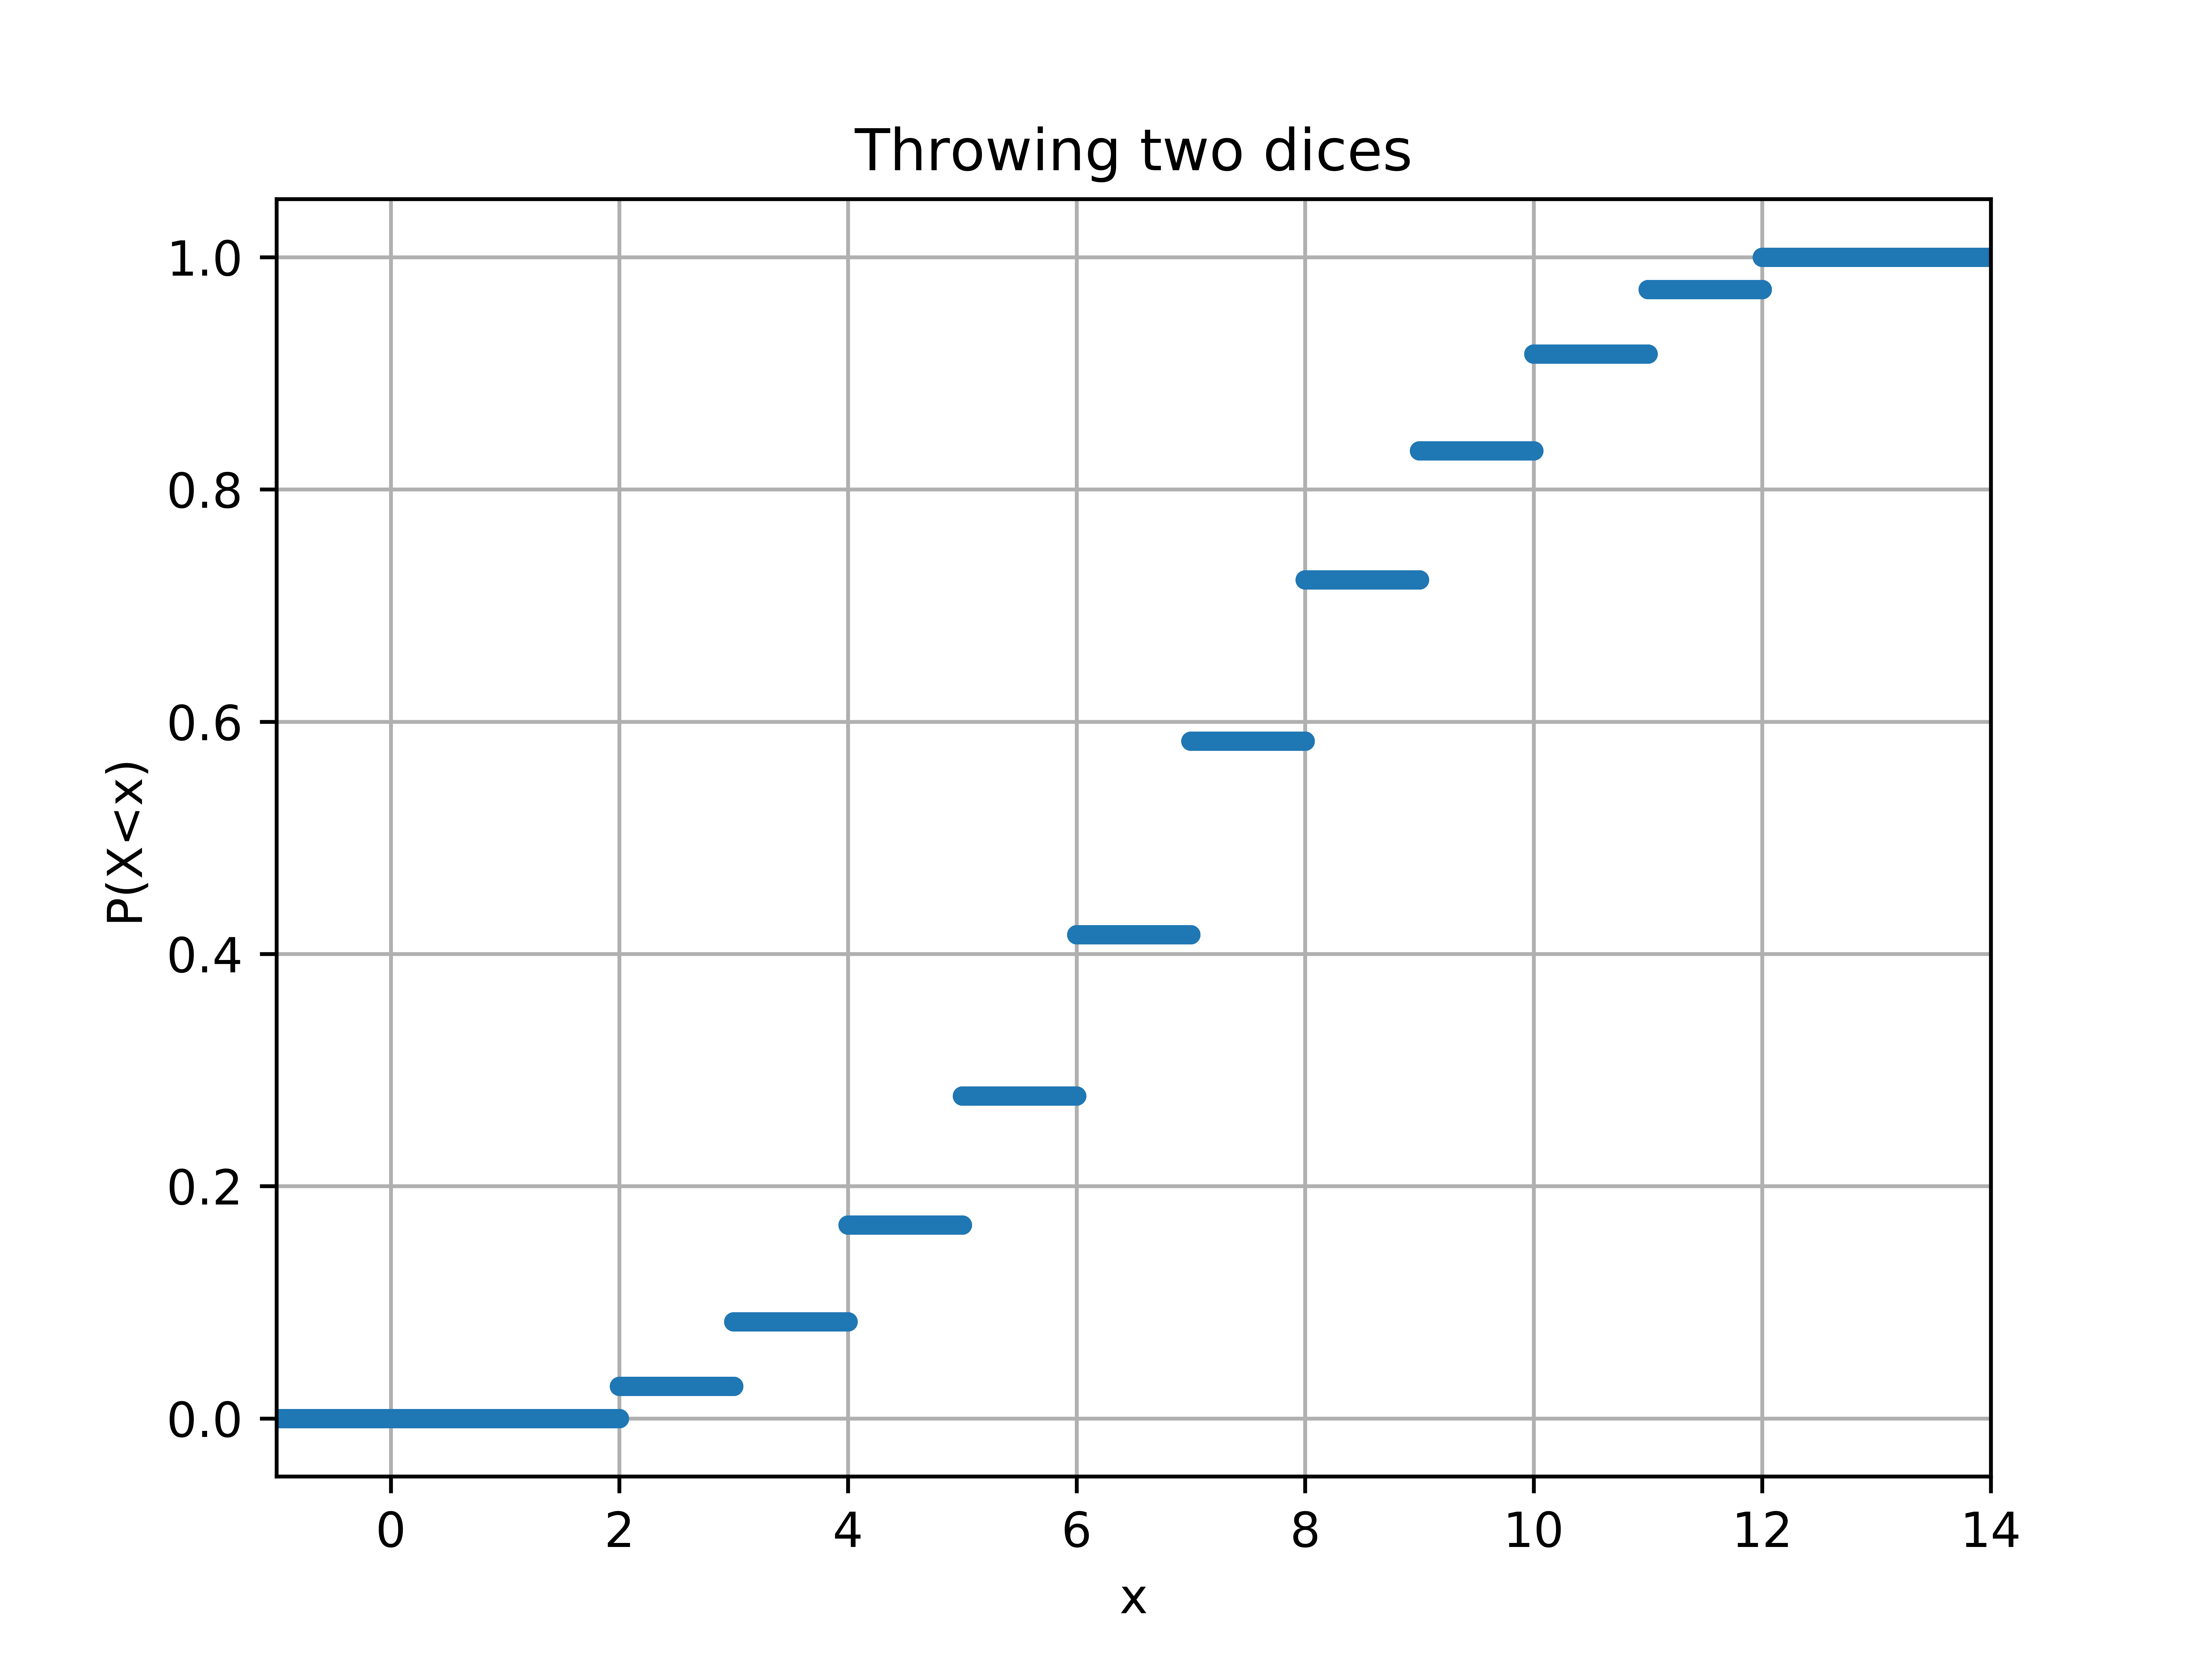
\includegraphics[width=0.5\linewidth]{./lect4/1.png}
\end{center}

\paragraph{Example} $\Omega = [0,2]$


\begin{center}
	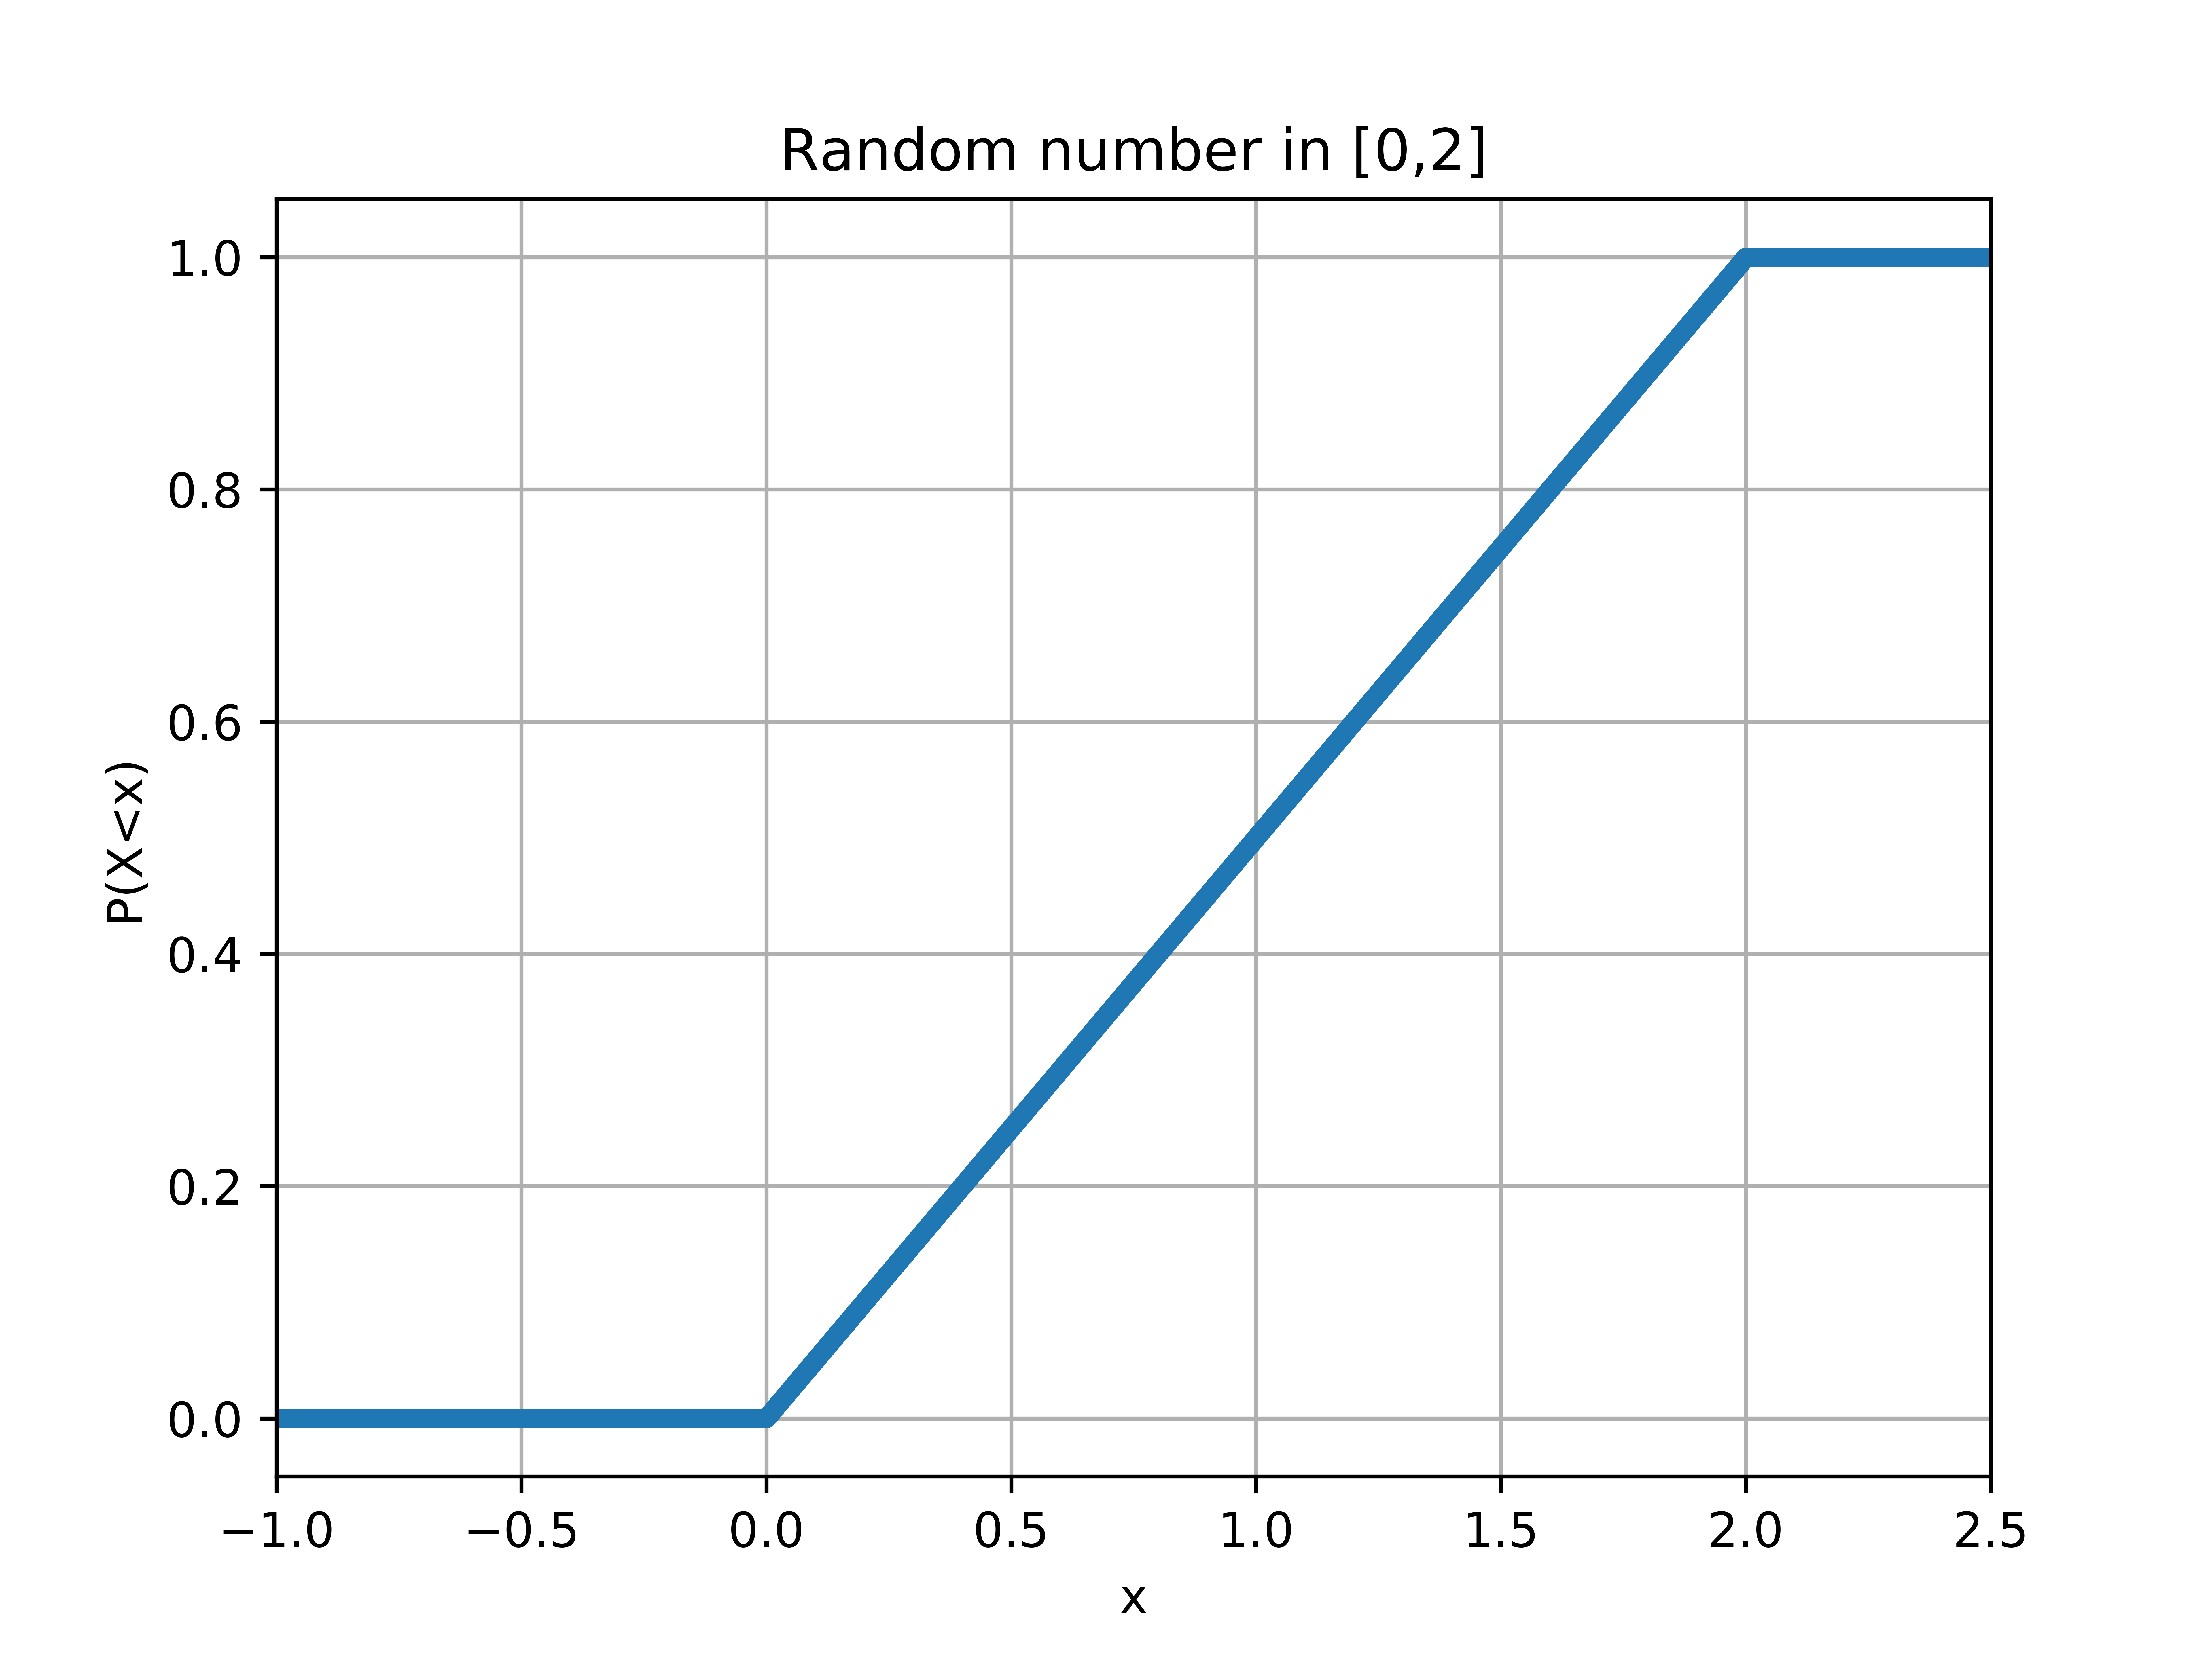
\includegraphics[width=0.5\linewidth]{./lect4/2.png}
\end{center}

\paragraph{Claim}
Let $F$ distribution function. 
\begin{enumerate}
	\item $F$ in monotonous non-decreasing
	\item $F$ is continuous to the right, i.e. $\lim_{y \to x^+} F(y) = F(x)$.
	\item $F(x^-) = \lim_{y \to x^-} F(y) = P(X<x)$
	\item $F(x) - F(x^-) = P(X=x)$
	\item $\lim_{x \to \infty} F(x) = 1$ and $\lim_{x \to -\infty} F(x) = 0$
\end{enumerate}
\subparagraph{Proof}
\begin{enumerate}
\item Obvious.
\item Denote $A = \left\{ X \leq x \right\}$ and $A_n= \left\{ X \leq x+\frac{1}{n} \right\}$. Then $P(A) = F(x)$ and $P(A_n) = F(x+\frac{1}{n})$. We need to show that
$$\lim_{n \to \infty} F(x+\frac{1}{n}) = F(x)$$
i.e.
$$\lim_{n \to \infty} P(A_n) = P(A)$$
Since $A = \bigcap A_n$, it's true.
\item Denote $B = \left\{ X < x \right\}$ and $B_n = \left\{ X - \frac{1}{n} \right\}$. That means
$$P(B_n) = F(x-\frac{1}{n})$$
Now we claim that 
$$B = \bigcap_{n=1}^\infty B_n$$
Since $\omega \in B \iff X(\omega) < x$ and $\omega \in B_n \iff X(\omega) \leq x - \frac{1}{n}$.
Since
$$\lim_{n \to \infty} F(x-\frac{1}{n}) = P(X<x) $$
from monotonousness
$$F(x^-) =  \lim_{y \to x^-} F(y) =\lim_{n \to \infty} F(x-\frac{1}{n})$$
\item Since $$\left\{ X \leq x \right\} = \left\{ X <x \right\} \cup \left\{  X  = x \right\}$$
$$P(X \leq x) = P(X < x) + P(X=x)$$
Thus
$$F(x) - F(X^-) = P(X=x)$$
\item Denote $C_n = \left\{ X \leq n \right\}$. Then
$$\bigcup_{n=1}^\infty  = \Omega$$
Then
$$\lim_{n \to \infty} F(n) = \lim_{n \to \infty} P(C_n) = P(\Omega) = 1$$
\end{enumerate}
\paragraph{Definition}
Random variable is called discrete if its distribution function is piecewise constant, i.e. is constant except countable set of points without accumulation points. Or, alternatively, if it can be written as a finite linear combination of indicator functions of intervals. 

In discrete case exists sequence $\left\{ x_j \right\}_{j=1}^N \subset \mathbb{R}$ and $\left\{ p_j \right\}_{j=1}^N$ for $1\leq N \leq \infty$ such that
$$P(X=x_j) =p_j$$ and $$\sum_j p_j = 1$$
\paragraph{Definition}
Random variable is called continuous if its distribution function is continuous. Thus
$P(X=x) = 0$

In this case we always assume that $F$ is piecewise continuously differentiable, i.e. its derivative piecewise continuous.Thus,
$$F(b) - F(a) = \int_a^b F^\prime(x) dx$$
Then we call $f(x) = F^\prime(X)$ a density function. And 
$$P(a\leq X \leq b) = \int_a^b f(x) dx$$
Then
$$F(x) = \int_{-\infty}^{x} f(t) dt$$
\paragraph{Expectation}  or expected value, denoted as $\mathbb{E}X$ and defined as
	$$\mathbb{E}X = \sum_{i=1}^{n} p_j x_j \text{ if } \sum_{i=1}^n p_i |x_i| < \infty $$ 
\paragraph{Function of random variable} Let $\Psi : \mathbb{R} \to \mathbb{R}$. Define $Y = \Psi(X)$. Then $Y$ is random variable too. Also, then $\mathbb{E}Y = \mathbb{E} \Psi(X) = \sum_{i=1}^{n} p_j \Psi(x_j)$

\paragraph{Variance} Lets look at
$$\sigma^2 = \mathbb{E} (X-\mathbb{E}X)^2 = \mathbb{E}(X-\mu)^2 = \sum_{k=1}^\infty p_j (x_j - \mu)^2$$
Variance measures at closeness of random variable to the expectation.

Standard deviation $\sigma$ is square root of variance.
Also

$$\sigma^2 = \sum_{k=1}^\infty p_j (x_j - \mu)^2 = \sum_{k=1}^\infty p_j x_j^2 -2\mu \sum_{k=1}^\infty p_jx_j + \mu^2 \sum_{k=1}^\infty p_j =  \mathbb{E}X^2 - 2\mu \cdot mu + \mu^2 = \mathbb{E}X^2 - \mu^2$$
i.e.
$$\sigma^2 = \mathbb{E}X^2 - (\mathbb{E}X)^2 = \mathbb{E}X^2 - \mu^2$$

\subsection{Classical discrete distributions}
\subsubsection{Binomial distribution}
Model:
\begin{enumerate}
	\item There are $n$ independent experiments (Bernoulli trials)
	\item There are two possible results (success and fail)
	\item In every experiment, probability of success is $p$.
\end{enumerate}
Denote
$$X  =\left\{ \parbox{2cm}{\centering \scriptsize number of successes} \right\}$$
Then
$$P(X=k) = \binom{n}{k} \cdot p^k (1-p)^{n-k}$$
We say that $X \sim Bin(n,p)$ and $\mathbb{E}X = np$.
Lets show that:
\begin{align*}
\mathbb{E}X = \sum_{k=0}^n k \binom{n}{k} p^k (1-p)^{n-k} = \sum_{k=1}^n k \frac{n!}{k!(n-k)!} p^k (1-p)^{n-k} =\\= \sum_{k=1}^n = \frac{n!}{(k-1)!(n-k)!} p^k (1-p)^{n-k} = np \sum_{k=1}^n \frac{(n-1)!}{(k-1)!(n-k)!} p^{k-1 }(1-p)^{n-k}
\end{align*}
Denote $j = k-1$
$$\mathbb{E}X= np \sum_{k=1}^n \frac{(n-1)!}{(k-1)!(n-k)!} p^{k-1 }(1-p)^{n-k} = np \sum_{j=0}^{n-1} \underbrace{\binom{n-1}{j}p^{j}(1-p)^{(n-1)-j}}_{\sim Bin(n-1,p) \Rightarrow 1} = np $$

\paragraph{Note} $\mathbb{E}X^n$ is $n^{th}$ moment of $X$
\paragraph{Variance of $X$}
Since $\mathbb{E}X = np$ and $Var(X) = \mathbb{E}X^2 - (\mathbb{E}X)^2 = \mathbb{E}X^2 - n^2p^2$
Lets calculate $\mathbb{E}X^2$:
$$\mathbb{E}X^2 = \sum_{k=0}^n k^2 \binom{n}{k} p^k (1-p)^{n-k} = \sum_{k=0}^n k(k-1) \binom{n}{k} p^k (1-p)^{n-k} + \underbrace{\sum_{k=0}^n k \binom{n}{k} p^k (1-p)^{n-k}}_{\mathbb{E}X}$$
\begin{align*}
\sum_{k=0}^n k(k-1) \binom{n}{k} p^k (1-p)^{n-k} =  \sum_{k=2}^n k(k-1) \frac{n!}{k!(n-k)!} p^k (1-p)^{n-k} =\\= \sum_{k=2}^n \frac{n!}{(k-2)!(n-k)!} p^k (1-p)^{n-k}  = n(n-1)p^2 \underbrace{\sum_{k=2}^n \frac{(n-2)!}{(k-2)!(n-k)!} p^{k-2 }(1-p)^{n-k}}_{\sim Bin(n-2,p) \Rightarrow 1} =  n(n-1)p^2 
\end{align*}
Then
$$Var(X) = n(n-1)p^2  + np - n^2p^2 = n^2p^2 +np- np^2 -n^2p^2 = np(1-p)$$


\subsubsection{Geometric distribution}
Performing Bernoulli trials until success. Define random variable
$$X = \left\{ \parbox{2cm}{\scriptsize \centering Number of required experimets} \right\}$$
$$P(X=n) = (1-p)^{n-1} p $$
$$X \sim Geom(p)$$
Then
$$\mathbb{E}X = \sum_{n=1}^\infty n(1-p)^{n-1}p $$

Lets use generating functions. Define $g(x) = \sum_{n=0}^\infty x^n = \frac{1}{1-x}$
Then $g^\prime(x) = \sum_{n=1}^\infty nx^{n-1} = \frac{1}{(1-x)^2}$
Then $g^\prime(1-p) = \sum_{n=1}^\infty n(1-p)^{n-1} = \frac{1}{p^2}$
i.e
$$\mathbb{E}X = \frac{p}{p^2} = \frac{1}{p}$$
Then
$$\mathbb{E}X^2 = \sum_{n=1}^\infty n^2(1-p)^{n-1}p = \sum_{n=2}^\infty n(n-1)(1-p)^{n-1}p+\frac{1}{p}$$
For same $g$, $g^{\prime\prime}(x) = \sum_{n=2}^\infty n(n-1)x^{n-2} = \frac{2}{(1-x)^3}$.
Substituting
$$\mathbb{E}X^2 = \sum_{n=2}^\infty n(n-1)(1-p)^{n-1}p+\frac{1}{p} = p(1-p) \cdot \frac{2}{p^3} + \frac{1}{p} =  \frac{2(1-p) }{p^2} + \frac{1}{p} = \frac{2}{p^2} - \frac{1}{p}$$
Thus
$$Var(X) = \frac{2}{p^2} - \frac{1}{p} - \frac{1}{p^2} = \frac{1-p}{p^2}$$
\paragraph{Lemma}
Let $X$ random variable with finite expectation. Then $\mathbb{E}(X+c) = \mathbb{E}X + c$ and $\mathbb{E}(cX) = c\mathbb{E}X$.
\subparagraph{Proof}
Define $Y= X+c$
Then
$$\mathbb{E}Y  = \sum p_i (x_i + c) = \sum p_i x_i + c\sum p_i = \mathbb{E}X+c $$
Similarly for $Z=cX$.
\paragraph{Lemma}
Let $X$ random variable with finite expectation. Then $Var(X+c) = Var(X)$ and $Var(cX) = c^2 Var(x)$.
\subparagraph{Proof}
Denote $Y = X+c$:
$$Var(Y) = \mathbb{E}(X+c - (\mathbb{E}X+c))^2 = \mathbb{E}(X-\mathbb{E}X)^2 = Var(X)$$
$Z=cX$:
$$Var(Z) = = E(\mathbb{E}X - c\mathbb{E}X)^2 = \mathbb{E}c^2(X-\mathbb{E}X)^2 = c^2 Var(X)$$

\subsubsection{Hypergeometric distribution}
There are $N$ balls in box, $m$ are ''good`` and $N-m$ are ''bad``. We take out $n$ balls out of box and count how much are good. There are $n$ Bernoulli trials. Probability that it every of them would be successful is $\frac{m}{N}$. But experiments aren't independent, so it's not binomial distribution.

We know that $0\leq k \leq m$ and $0\leq n-k \leq N-m$. Thus $$\max (0, n+m-N) \leq k \leq \min(m,n)$$
For $k$ in this range
$$P(X=k) = \frac{\binom{m}{k}\binom{N-m}{n-k}}{\binom{N}{n}}$$

For hypergeometric distribution:
$$EX = \frac{nm}{N}$$
$$Var(X) = n \frac{m}{N}\left(1-\frac{m}{N}\right) \frac{N-n}{N-1}$$

In limit of $N,m \to \infty$ and $\frac{m}{N} \to p$, then for fixed $n$, we get back the binomial distribution.
\subsubsection{Poisson distribution}
$$P(X=k) = \frac{\lambda^k}{k!} e^{-\lambda}$$
$$X \sim Pois(\lambda)$$
Then $\mathbb{E} X = \sigma^2(X) = \lambda$.
\paragraph{Theorem (Poisson approximation of binomial distribution)}
$$\lim_{n \to \infty \: p \to 0 \: np \to \lambda} \binom{n}{k}p^k (1-p)^{n-k} = \frac{\lambda^k}{k!} e^{-\lambda}$$
If $X_{n,p} \sim Bin(n,p) $ and $X_\lambda \sim Pois(\lambda)$ then
$$\lim_{n \to \infty \: p \to 0 \: np \to \lambda} P(X_{n,p}=k)  = P(X_\lambda = k) $$

\subparagraph{Proof}
We can rewrite $p_n = \frac{\lambda + \delta_n}{n}$, where $\delta_n \to 0$
Let $k \in \mathbb{N}$ and $n\geq k$
\begin{align*}
\binom{n}{k}p_n^k (1-p_n)^{n-k} = \frac{n(n-1)\dots (n-k+1)}{k!} \left(\frac{\lambda + \delta_n}{n}\right)^k \left(1-\frac{\lambda + \delta_n}{n}\right)^{n-k} = \frac{n(n-1)\dots (n-k+1)}{k!} \frac{ \left(\lambda + \delta_n\right)^k }{n^k } \frac{\left(1-\frac{\lambda + \delta_n}{n}\right)^{n}}{\left(1-\frac{\lambda + \delta_n}{n}\right)^{k}} =\\=\underbrace{ \frac{n(n-1)\dots (n-k+1)}{n^k}  }_{1}\frac{1}{k!}\underbrace{\left(\lambda + \delta_n\right)^k}_{\lambda^k}\underbrace{ \left(1-\frac{\lambda + \delta_n}{n}\right)^{n}}_{e^{-\lambda}} \underbrace{ \frac{1}{\left(1-\frac{\lambda + \delta_n}{n}\right)^{k}}}_{1} = \frac{\lambda^k}{k!} e^{-\lambda}	
\end{align*}

$$\mathbb{E}X = \sum_{k=1}^\infty k \frac{\lambda^k}{k!} e^{-\lambda}  = e^{-\lambda}\lambda \sum_{k=1}^\infty  \frac{\lambda^{k-1}}{(k-1)!} =e^{-\lambda} \lambda e^{\lambda} = \lambda  $$
$$\mathbb{E}X^2 = \sum_{k=1}^\infty k^2 \frac{\lambda^k}{k!} e^{-\lambda} = e^{-\lambda}\left[\sum_{k=1}^\infty \left(k(k-1) + k\right) \frac{\lambda^k}{k!} \right] = \lambda^2 + \lambda$$
$$\sigma^2(X) = \lambda$$

\subsubsection{Uniform distribution on $[n] = \left\{ 1,2,\dots, n \right\}$}

\paragraph{Example of infinite expectation}
$$P(X = 2^n) = 2^{-n}$$
The model is flipping coin until you get head and getting $2^n$ dollars where $n$ is number of flips you made.
Then expectancy of your profit
$$EX = \sum 2^n 2^{-n} = \infty$$

\section{ Continuous random variables}
Since $f(x) = F^\prime(x)$
$$\int_{-\infty}^{\infty} f(x) dx = 1$$
We define expectation of $X$ as
$$\mu = \mathbb{E}X = \int_{-\infty}^{\infty} xf(x) dx$$
We can define expectation in broad sense. If one of $\int_{-\infty}^0 xf(x) dx$ and $\int_0^\infty xf(x) dx$ is finite and second is infinite, we can define expectation as infinite.

 \subsection{Function of continuous of random variable}
 For $X: \Omega \to \mathbb{R}$ define 
 $$Y = \Psi(X)$$
 Then
 $$\mathbb{E}Y = \mathbb{E} \Psi(X) = \int_{-\infty}^\infty = \int_{-\infty}^\infty \Psi(x) f(x) dx$$
Now we can use it to define variance, by using $\psi(x) = (x-\mu)^2$:
$$\sigma^2 = \mathbb{E}(X-\mu)^2 = \int_{-\infty}^\infty (x-\mu)^2 f(x)dx$$

\paragraph{Claim}
$$\sigma^2(X) = \mathbb{E}X^2 - (\mathbb{E}X)^2$$
\subparagraph{Proof}
$$\sigma^2(X) = \int_{-\infty}^\infty  (x-\mu)^2 f(x) dx =\int_{-\infty}^\infty x^2 f(x) dx-2\mu \int_{-\infty}^\infty  \underbrace{x f(x)}_{\mu} dx+\mu^2\underbrace{\int_{-\infty}^\infty  f(x) dx}_{1} = EX^2-\mu^2$$

\subsection{Classical continuous distributions}
\subsubsection{Uniform distribution}
For $[a,b]$:
$$f(x) = \begin{cases}
\frac{1}{b-a}&  a \leq x\leq b\\0& otherwise
\end{cases}$$

$$EX = \frac{b+a}{2}$$
We write $X \sim U\big( [a,b] \big)$.

\begin{center}	
	\includesvg[eps,svgpath = lect9/,width=0.5\linewidth]{uniform}
\end{center}
\subsubsection{Exponential distribution}
For $\lambda > 0$
$$f(x) = \lambda e^{-\lambda x}, \: x \geq 0$$
Then $$F(x) = \int_{-\infty}^x f(t) dt = \int_0^x f(x) dt = 1-e^{-\lambda x}$$
$$EX = \int_0^\infty x \lambda e^{-\lambda x} dx = \left[ -xe^{-\lambda x} \right]_0^\infty + \int_0^\infty e^{-\lambda x}dx = \frac{1}{\lambda }$$
$$\sigma^2 = EX^2 - (EX)^2 = EX^2 - \left(\frac{1}{\lambda}\right)^2 = \frac{1}{\lambda^2} $$

\begin{center}	
	\includesvg[eps,svgpath = lect9/,width=0.5\linewidth]{exp}
\end{center}

If $X \sim Exp(\lambda)$ then 
$$P(X \geq a+b | X\geq a) = P(X \geq b)$$
This property is called memorylessness.
\paragraph{Proof that exponential distribution is memoryless}
$$P(X \geq a+b | X \geq a)= \frac{P(X \geq a+b, \: X \geq a)}{P(X \geq a)}= \frac{P(X \geq a+b) }{P(X \geq a)} = \frac{e^{-\lambda(a+b)}}{e^{-\lambda a}}=e^{-\lambda b}$$ 
\paragraph{Notation}
$P(A,B) = P(A \cap B)$
\paragraph{Model}
For example, the time until a radioactive particle decays or time until you get cellphone call.


\subsubsection{Normal (Gaussian) distribution}
\paragraph{Proof of integral}
Denote $$l =  \int_{-\infty}^\infty  e^{-\frac{x^2}{2}}dx$$
Since $l$ is even;
$$\frac{l}{2} =  \int_{0}^\infty  e^{-\frac{x^2}{2}}dx$$
Now
$$\frac{l^2}{4} =  \int_{0}^\infty  e^{-\frac{x^2}{2}}dx\int_{0}^\infty  e^{-\frac{y^2}{2}}dy = \int_{0}^\infty \int_{0}^\infty  e^{-\frac{x^2+y^2}{2}}dxdy$$
The integral is in first quarter. Switching to polar:
$$dxdy = rdr d\theta$$
$$\frac{l^2}{4}  = \int_{0}^\infty \int_{0}^\infty  e^{-\frac{x^2+y^2}{2}}dxdy = \int_0^\frac{\pi}{2} d\theta \int_0^\infty dr re^{-\frac{r^2}{2}} =  \int_0^\frac{\pi}{2} d\theta \left[ -e^{-\frac{r^2}{2}} \right]_0^\infty =  \int_0^\frac{\pi}{2} = \frac{\pi}{2}$$
$l = \sqrt{2\pi}$
\paragraph{Normal distribution}
$$f(x) = c e^{-\frac{(x-a)^2}{2b}}$$
$$\int_{-\infty}^\infty f(x) = c \int_{-\infty}^\infty  e^{-\frac{(x-a)^2}{2b}} = 1$$
Substitute $z = \frac{x-a}{\sqrt{b}}$ and $dx = \sqrt{b}dz$.

$$c \int_{-\infty}^\infty  e^{-\frac{(x-a)^2}{2b}} = c\sqrt{b} \int_{-\infty}^\infty  e^{-\frac{z^2}{2}}dz c\sqrt{2\pi b}$$
Then
$$c = \frac{1}{\sqrt{2\pi b}}$$
and
$$f(x) = \frac{1}{\sqrt{2\pi b}} e^{-\frac{(x-a)^2}{2b}}$$
which is density function.
\paragraph{Expectation of normal distribution}
$$\int_{-\infty}^\infty x f(x) dx = \int_{-\infty}^\infty x f(x)\frac{e^{-\frac{(x-a)^2}{2b}}}{\sqrt{2\pi b}}  dx =  \underbrace{\int_{-\infty}^\infty (x-a) f(x)\frac{e^{-\frac{(x-a)^2}{2b}}}{\sqrt{2\pi b}}  dx}_{\text{odd function} \Rightarrow =0} + \int_{-\infty}^\infty a f(x)\frac{e^{-\frac{(x-a)^2}{2b}}}{\sqrt{2\pi b}}  dx = a\int_{-\infty}^\infty  f(x)\frac{e^{-\frac{(x-a)^2}{2b}}}{\sqrt{2\pi b}}  dx = a$$
Since $a$ is mean, we'll replace it with $\mu$:
$$f(x) = \frac{e^{-\frac{(x-\mu)^2}{2b}}}{\sqrt{2\pi b}} $$


\paragraph{Variance of normal distribution}
$$\int_{-\infty}^\infty z^2 e^{-\frac{z^2}{2}} dz $$
By parts: $u=z$ and $v^\prime = ze^{-\frac{z^2}{2}}$. Then
$$\int_{-\infty}^\infty z^2 e^{-\frac{z^2}{2}} dz = \left[ -z  e^{-\frac{z^2}{2}} \right]_{-\infty}^\infty + \int_{-\infty}^\infty e^{-\frac{z^2}{2}} dz = \sqrt{2 \pi}$$
lets calculate variance:
$$\sigma^2 = \int_{-\infty}^\infty (x-\mu)^2 \frac{e^{-\frac{(x-\mu)^2}{2b}}}{\sqrt{2\pi b}} dx$$
With same substitution  $z = \frac{x-\mu}{\sqrt{b}}$:
$$\sigma^2 = \int_{-\infty}^\infty bz^2 \frac{e^{-\frac{z^2}{2}}}{\sqrt{2\pi}} dz =b \underbrace{\int_{-\infty}^\infty z^2 \frac{e^{-\frac{z^2}{2}}}{\sqrt{2\pi}} dz}_{1} = b $$
Thus $\sqrt{b} = \sigma$.

Which leads us to final form of $f(x)$:
$$f(x) = \frac{e^{-\frac{(x-\mu)^2}{2\sigma^2}}}{\sqrt{2\pi}\sigma} $$
We write $X \sim N(\mu, \sigma^2)$.

\begin{center}	
	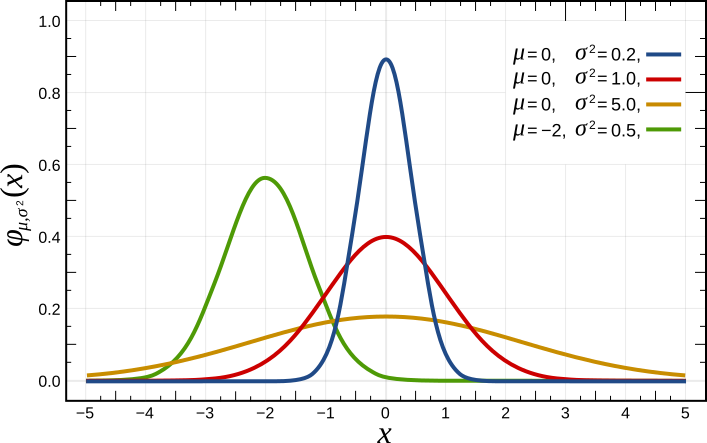
\includegraphics[width=0.5\linewidth]{./lect9/norm.png}
\end{center}
It can be shown that $x = \mu \pm \sigma$ are inflection point.

$$F(x) = \int_{-\infty}^{x} \frac{e^{-\frac{(y-\mu)^2}{2\sigma^2}}}{\sqrt{2\pi} \sigma} dy$$

Lets denote $Z \sim N(0,1)$ is standard distribution. Canonical substitution   $z = \frac{x-\mu}{\sigma}$:
For $\mu \in \mathbb{R}$ and $\sigma^2 >0 $, we can show $P(\mu + a \sigma \leq X \leq \mu + b \sigma)$ is independent on $a$ and $b$:
$$P(\mu + a \sigma \leq X \leq \mu + b \sigma) = \int_{\mu + a \sigma}^{\mu + b \sigma} \frac{e^{-\frac{(x-\mu)^2}{2\sigma^2}}}{\sqrt{2\pi} \sigma} dx = \int_{a}^{b} \frac{e^{-\frac{z^2}{2}}}{\sqrt{2\pi} } dx = P(a\leq Z \leq b)$$

\paragraph{Conclusion}
$$\frac{X_{\mu, \sigma^2} - \mu}{\sigma} = Z$$

\paragraph{Claim}
Suppose $X$ random variable such that $\exists a,b \quad -\infty \leq a < b \leq  \infty$ $\forall x \notin [a,b] \quad f_X(x) = 0$ .

Let $\Psi : [a,b] \to \mathbb{R}$ continuous, monotonous, piecewise continuously differentiable. Define $Y = \Psi(X)$, then $Y$ is continuous random variable and
$$f_Y(y) = \frac{f_X(x)}{|\Psi^\prime (x)|} =\frac{f_X(\Psi^{-1}(y))}{|\Psi^\prime (\Psi^{-1}(y))|}  $$ 
\subparagraph{Proof}
Without loss of generality, $\Psi$ is decreasing.
$$F_Y(y) = P(Y \leq y)  = P(\Psi(X) \leq y) = P(X \geq \Psi^{-1}(y))  = 1 - P(X \leq \Psi^{-1}(y)) = 1 -  F_X(\Psi^{-1}(y)) = 1 - F_X(\Psi^{-1}(y))$$
Thus
$$f_Y(y) = F_Y^\prime(y) = -(F_X(\Psi^{-1}(y))) = -F^\prime_X(\Psi^{-1}(y)) \cdot \left( \Psi^{-1}(y) \right)^\prime$$

Since $\left(\Psi^{-1}\right)^\prime(y) = \frac{1}{\Psi^\prime (\Psi^{-1}(y))}$:
$$f_Y(y) = -f_X (\Psi^{-1}(y)) \cdot\frac{1}{\Psi^\prime (\Psi^{-1}(y))} = \frac{f_X(x)}{|\Psi^\prime(x)|} $$

\paragraph{Claim}
Let $\psi$ piecewise monotonous, i.e. consists of finite or countable intervals in each of which its monotonous, then
$$f_Y(y) = \sum_{x: \psi(x)=y} \frac{f_X(x)}{|\psi^\prime(x)|}$$

\paragraph{Simulation}
$$U \sim U \left( [0,1] \right)$$
$$F_U(x) = \begin{cases}
0,&x<0\\
x,&0\leq x\leq 1\\
1,&x>1
\end{cases}$$
$$f_U(x) = 1, \: 0\leq x \leq 1$$

To acquire a number which is distributed (approximately) by $U$:

Choose $n \in N$, toss a coin $n$ times and write down a number as binary:
$0.a_1a_2a_3\dots a_n$. 

\paragraph{Claim} Let $X$ continuous random variable with distribution function $F_X$. Suppose $\exists -\infty \leq a < b \leq -\infty$ such that $F_x(a) = 0 $ and $F_x(b) = 1$, such that $F_X$ is completely monotonic on $(a,b)$. Suppose $U \sim U\big( [0,1] \big)$ and define $Y  =F_X^{-1}(U)$ then $Y \sim X$.
\subparagraph{Proof}
$$F_Y(y) = P(Y \leq y)= P(F_X^{-1}(U) \leq y) = P(U \leq F_X(y)) = F_U(F_X(y)) = F_X(y)$$
\paragraph{Example}
$$X \sim Exp(\lambda)$$
$$f_X(x) = \lambda e^{-\lambda x}$$
$$F_X(x) = \begin{cases}
0,&x<0\\1-e^{-\lambda x},& x \geq 0
\end{cases}$$
Lets find $F^{-1}_X(y) $
$$y = 1-e^{-\lambda x}$$
$$-\lambda x = \log (1-y)$$
$$ x = -\frac{ \log (1-y)}{\lambda}$$
Thus
$$F^{-1}_X(y) =  -\frac{1}{\lambda} \log (1-y)$$
Thus we define
$$Y = -\frac{1}{\lambda} \log (1-U)$$
and $Y \sim X$.
\\

\paragraph{Claim} Suppose $F_X$ is completely monotonic and piecewise continuously differentiable. Then $Y=F_X(X) \sim U([0,1])$. 
\subparagraph{Proof}
$$F_Y(y) = P(Y \leq y)= P(F_X(X) \leq y) = P(X \leq F_X^{-1}(y)) = F_X(F_X^{-1}(y)) = y$$

\paragraph{Note}
$$X = X^+ + X^-$$
$$\mathbb{E}X^+= \begin{cases}
\sum_{j: x_j > 0} p_j e^{tx_j} & \text{discrete}\\
\int_{0}^\infty  e^{tx}f(x) dx & \text{continuous}
\end{cases}$$
$$\mathbb{E}X^+= \begin{cases}
-\sum_{j: x_j < 0} p_j e^{tx_j} & \text{discrete}\\
-\int_{-\infty}^0  e^{tx}f(x) dx & \text{continuous}
\end{cases}$$


\paragraph{Moment-generating function}
$$M_X(t) = \mathbb{E} e^{tX}$$
Obviously $M(0) = 1$.
Generally:
$$M_X(t) = \begin{cases}
\sum_{j=1}^N p_j e^{tx_j} & \text{discrete}\\
\int_{-\infty}^\infty  e^{tx}f(x) dx & \text{continuous}
\end{cases}$$

Now, if $\mathbb{E} (X^+)^n = \infty$, then $\forall t>0 \quad M_X(t) = \infty$, and if $\mathbb{E} (X^-)^n = \infty$, then $\forall t<0 \quad M_X(t) = \infty$.

That means that necessary condition for existence of $M_X$ in neighborhood of $0$ is $\mathbb{E} |X|^n < \infty$.
\paragraph{Note}
If $M_X(t) < \infty$ for $t$ in neighborhood of $t_0$, then $M_X$ if differentible infinite times and 
$$\frac{d^n}{dt^n} M_X(t) = \mathbb{E} X^n e^{tX}$$  
In particular,
$$\frac{d^n}{dt^n} M_X(0) = \mathbb{E} X^n$$
By Taylor
$$M_X(t) = \sum_{n=0}^\infty \frac{M_X^{(n)}(0)}{n!}t^n$$  
\paragraph{Example}
$$X \sim N(0,1)$$
$$f(x) = \frac{e^{-\frac{x^2}{2}}}{\sqrt{2} \pi}$$
$$M_X(t) = \int_{-\infty}^{\infty} e^{tx} \frac{e^{-\frac{x^2}{2}}}{\sqrt{2} \pi} dx = e^{\frac{t^2}{2}}\int_{-\infty}^{\infty} \frac{e^{-\frac{(x-t)^2}{2}}}{\sqrt{2} \pi} dx = e^{\frac{t^2}{2}}$$
Thus
$$M_X(t) = \sum_{n=0}^\infty \frac{t^{2n}}{2^nn!} = \sum_{n=0}^\infty \frac{(2n)!}{2^nn!} \frac{t^{2n}}{(2n!)}$$
That means
$$\mathbb{E} X^{2n+1} =0$$
(that can be seen from direct calculation, acquiring integral of odd function on whole $\mathbb{R}$)
$$\mathbb{E} X^{2n} = \frac{(2n)!}{2^n} = \frac{2n(2n-1)(2n-2)(2n-3)\dots 1}{2^n n(n-1)(n-2)\dots 1} =  \frac{2^n \cdot n(2n-1)(n-1)(2n-3)(n-2)\dots 1}{2^n n(n-1)(n-2)\dots 1} = (2n-1)(2n-3)(2n-5)\dots \cdot 5 \cdot 3 \cdot 1 $$
\section{Markov's and Chebyshev's inequalities}
\paragraph{Markov's inequality }
Let $Y\geq 0$ and $\mathbb{E} Y < \infty$. Then,
$$\forall \lambda > 0 \quad P(Y \geq \lambda) \leq \frac{\mathbb{E} Y}{\lambda}$$
\subparagraph{Proof}
Discrete:
$$P(Y \geq \lambda) = \sum_{j: y_j > \lambda} p_j \leq \sum_{j: y_j > \lambda} \frac{y_j}{\lambda} p_j  \leq \frac{1}{\lambda} \sum_j p_jy_j = \frac{\mathbb{E} Y}{\lambda}$$
Continuous:
$$P(Y \geq \lambda) = \int_\lambda^\infty f(y) dy \leq \int_\lambda^\infty \frac{y}{\lambda}f(y) dy   \leq \frac{1}{\lambda}\int_0^\infty yf(y)dy = \frac{\mathbb{E} Y}{\lambda}$$
\paragraph{Chebyshev's inequality}
Let $X$ random variable for which second moment exists. Denote $\mu = \mathbb{E} X$ and $\sigma^2 = Var(x)$ then
$$P(|X-\mu| \geq \lambda) \leq \frac{\sigma^2}{\lambda^2}$$

\subparagraph{Proof}
Define $Y = (X-\mu)^2$
By Markov inequality:
$$P(|X-\mu|\geq \lambda) = P\left( (X-\mu)^2 \geq \lambda^2 \right) = P\left( Y^2 \geq \lambda^2 \right) \leq \frac{1}{\lambda^2} \mathbb{E} Y = \frac{\mathbb{E} (X-\mu)^2}{\lambda^2} = \frac{\sigma^2}{\lambda^2}$$
\section{Multiple random variable}
\paragraph{Random vector}
Let $X$ and $Y$ two random variables on same probability space. Then $(X,Y)$ is random vector. Define
$$F(x,y) = P(X \leq x, Y \leq y)$$
which is called joint distribution function.
\paragraph{Claim}
\begin{enumerate}
	\item  $F$ is monotonic in both $x$ and $y$.
	\item  $\lim_{x\to -\infty} F(x,y)=\lim_{y\to -\infty} F(x,y) = 0$.
	\item  $\lim_{x\to \infty} F(x,y)= F_Y(y)$
	
	$\lim_{y\to \infty} F(x,y) = F_X(x)$.
	
	$F_X$ and $F_Y$ are called marginal distribution function.
	\item  $\lim_{x\to \infty, y\to \infty} F(x,y)= 1$
	
	\item  $F$ is continuous from the right for both of $x$ and $y$.
\end{enumerate}
\paragraph{Claim}
$$-\infty \leq a < b \leq +\infty$$
$$-\infty \leq c < d \leq +\infty$$

Then
$$P(a<X\leq b, c < Y \leq d) = F(b,d) - F(b,c) - F(a,b) + F(a,c)$$


\paragraph{Discrete vector}
$F(x,y)$ is piecewise constant. In other words, $X$,$Y$ are discrete random variables:
$$P(X=x_i) = p_i^X : p_i^X > 0$$
$$P(Y=y_j) = p_j^Y : p_j^Y > 0$$
and
$$P\Big((X,Y) = (x_i, y_j)\Big)  = P(X=x_i, Y=y_j) = p_{ij}: p_{ij} \geq 0$$

Then we can write
$$p_i^X = P(X=x_i) = \sum_{j=1}^m p_{ij}$$
$$p_j^Y = P(Y=y_i) = \sum_{i=1}^n p_{ij}$$

Now if we take the previous equation:
$$P(a<X \leq b , c < Y \leq d) = F(b,d)-F(a,d) -F(b,c)-F(a,c)$$
Then if $a \to b$ and $c \to d$:
\begin{align*}
P\Big((X,Y) = (b,d)\Big) = P(a<X \leq b , c < Y \leq d) = F(b,d)-F(b^-,d) -F(b,d^-)+F(b^-, d^-) =\\= \big( F(b,d)-F(b^-,d) \big) - \big( F(b,d^-)-F(b^-, d^-)  \big)
\end{align*}

\paragraph{Continuous variable}
$F(x,y)$ continuous in both $x$ and $y$. We always suppose that $F$ is piecewise twice differentiable and define
$$f(x,y) = \frac{\partial^2 F}{\partial x \partial y}$$
Then
\begin{align*}
\int_a^b \int_c^d f(x,y) dxdy = \int_a^b dx \int_c^d dy \frac{\partial}{\partial y} \left( \frac{\partial F}{\partial x} \right) (x,y)  =\\= \int_a^b dx \left(\frac{\partial F}{\partial x}(x,d) - \frac{\partial F}{\partial x}(x,b)\right) = F(b,d) -F(a,d) - F(b,c) + F(a,c) = P(a<X \leq b , c < Y \leq d)
\end{align*}
\paragraph{Lemma}
Suppose $h$, $g$ integrable on $(c,d)$, $-\infty \leq c < d \leq \infty$. Suppose
$$\forall c \leq a < b \leq d \int_a^b g(x) dx = \int_a^b h(x) dx$$
Then if $g$ and $h$ is continuous, $g(x) = h(x)$.
\subparagraph{Proof}
Suppose $x \in (c,d)$ such that $g$ and $h$ continuous.
$$\forall d-x > \delta > 0 \quad \int_x^{x+\delta} g(y) dy = \int_x^{x+\delta} h(y) dy  $$
$$\frac{1}{\delta}\int_x^{x+\delta} g(y) dy =\frac{1}{\delta} \int_x^{x+\delta} h(y) dy $$
In limit $\delta \to 0$, for continuous functions $g(x)=h(x)$.
\paragraph{Claim} 
$$\int_{-\infty}^{\infty} f(x,y) dy = f_X(x)$$
and
$$\int_{-\infty}^{\infty} f(x,y) dx = f_Y(y)$$

\subparagraph{Proof}
For $-\infty \leq a < b \leq \infty $ and  $-\infty \leq c < d \leq \infty $:
$$P(a\leq X\leq b, c \leq Y \leq d) = \int_c^d \int _a^b f(x,y) dx dy$$
In limit $c \to -\infty$, $d \to \infty$:
$$P(a\leq X\leq b) = \int_{-\infty}^\infty dy \int _a^b f(x,y) dx = \int _a^b  \int_{-\infty}^\infty  f(x,y) dy  dx $$
But
$$P(a\leq X\leq b) = \int_a^b f_X(x) dx$$
Then
$$\int _a^b  \int_{-\infty}^\infty  f(x,y) dy  dx  = \int_a^b f_X(x) dx$$
From lemma
$$ \int_{-\infty}^\infty  f(x,y) dy  = f_X(x)$$

\paragraph{Generalization}
$$P\big( (X,Y) \in A \big) = \int_a^b dx \int_c^d dy f(x,y) = \iint\limits_A f(x,y) dx dy$$

\paragraph{Dimension reduction}
$$\Psi: \mathbb{R}^2 \to \mathbb{R}$$
\subparagraph{Discrete}
$$\mathbb{E} \Psi(X,Y) = \sum_{i=1}^n \sum_{j=1}^m \Psi(x_i, y_j) p_{ij} $$
\subparagraph{Continuous}
$$\mathbb{E} \Psi(X,Y) = \int_{-\infty}^\infty\int_{-\infty}^\infty \Psi(x,y)f(x,y) dxdy$$
\paragraph{Example}
$\Psi(x,y) =  \mathds{1}_A$.

Then

$$\mathbb{E} \Psi(X,Y) = \int_{-\infty}^\infty\int_{-\infty}^\infty \Psi(x,y) dxdy = \iint\limits_{A} f(x,y) dx dy = P\big((X,Y) \in A\big)$$
\paragraph{Example}
$$\Psi(x,y) = x$$
Obviously
$$\mathbb{E} \Psi(X,Y) = \mathbb{E} X$$
Formally:
$$\mathbb{E} \Psi(X,Y) = \int_{-\infty}^\infty\int_{-\infty}^\infty x f(x,y) dx dy = \int_{-\infty}^\infty x \int_{-\infty}^\infty  f(x,y)  dy dx = \int_{-\infty}^\infty xf_X(x) dx = \mathbb{E}X$$

\paragraph{Note} Everything said is naturally generalized to $N$ dimensions.
\subsection{Independence}
\paragraph{Definition}
$X$ and $Y$ are independent, if
$$P\big( a < X \leq b, c < Y \leq d \big) = P\big( a < X \leq b\big) P\big(c < Y \leq d \big)$$
Which is also generalized to any pair of (measurable)  set:
$$P(X \in A, Y \in B) = P(X \in A)P(Y \in B)$$

\paragraph{Claim}
The following 3 are equivalent:
\begin{enumerate}
	\item X and Y are independent
	\item $$F(x,y) = F_X(x)F_Y(y)$$
	\item $$p_{ij} = p_i^Xp_j^Y$$
	or 
	$$f(x,y) = f_X(x)f_Y(y)$$
	for discrete and continuous respectively.
\end{enumerate}
\subparagraph{Proof}
\begin{enumerate}
	\item $1 \Rightarrow 2$
	Immediate. For $a=c=-\infty$ and $b=x$, $d=y$:
	$$F(x,y) = P \left( X \leq x, Y \leq y \right) = P(X \leq x) P(Y \leq y) = F_X(x) F_Y(y)$$
	
	\item $1 \Leftarrow 2$
	\begin{align*}
	P(a<X \leq b , c < Y \leq d) = F(b,d) -F(a,d) - F(b,c) + F(a,c) =\\= F_X(b)F_Y(d) - F_X(a) F_Y(d) - F_X(b) F_Y(c) + F_X(a) F_Y(c) =\\= F_Y(d) \left( F_X(b)-F_X(a) \right) -  F_Y(c) \left( F_X(b)-F_X(a) \right) =  \left(F_Y(d)-  F_Y(c)\right) \left( F_X(b)-F_X(a) \right)  = P(a<X\leq b) P(c < Y\leq d)
	\end{align*}
	\item $2 \Rightarrow 3$ (continuous)
	$$F(x,y) = F_X(x)F_Y(y)$$
	$$\frac{\partial^2 F(x,y)}{\partial xy} = \frac{\partial^2 }{\partial xy} F_X(x)F_Y(y)$$
	$$f(x,y) = F^\prime_X(x)F_Y^\prime(y) = f_X(x)f_Y(y)$$
	\item $2 \Leftarrow 3$ (continuous)
	$$F(x,y) = \int_{-\infty}^x \int_{-\infty}^y f(x,y)dxdy = \int_{-\infty}^x \int_{-\infty}^y f_X(x)f_Y(y) dxdy =  \int_{-\infty}^x  f_X(x) dx \int_{-\infty}^yf_Y(y) dy =F_X(x) F_Y(y)$$
\end{enumerate}
\section{Conditional distribution}
\subsection{Discrete case}
$$p_{Y|X}(y|x) = P(Y=y|X=x) = \frac{P(X=x,Y=y)}{P(X=x)} = \frac{p(x,y)}{p_X(x)}$$
We'll call it distribution function. The definition is consistent:

$$\sum_y p_{Y|X}(y|x) = P(Y=y|X=x) = \sum_y \frac{p(x,y)}{p_X(x)} = 1$$

$$F_{Y|X=x} = P\left( Y \leq y|X=x \right) = \sum_{y^\prime \leq y} P\left( Y = y^\prime |X=x \right) = \sum_{y^\prime \leq y} p_{Y|X=x}\left(y^\prime |x \right) = \frac{1}{p(x)} \sum_{y^\prime \leq y} p\left(x, y^\prime  \right)$$
$$\mathbb{E} (Y|X=x) = \sum_y y p_{Y|X}(y|x) = \sum_y y \frac{p(x,y)}{p_X(x)} = \frac{1}{p_X(x)} \sum_y y p(x,y)$$
$$\mathbb{E} \big(\Psi(Y)|X=x\big) = \sum_y \Psi(y) p_{Y|X}(y|x)$$

\paragraph{Example}
$$X \sim Pois(\lambda)$$
$$Y|X=x  \sim Bin(x,p)$$
Find distribution of $Y$
\subparagraph{Solution}
$$P(Y=y) = \sum_x P(X=x,Y=y) = \sum_x P(X=x) P(Y=y|X=x) $$
or
$$P(Y=y) = \sum_x p(x,y) = \sum_x p_X(x) p_{Y|X} (y|x)$$

Now
$$P(X=x) = \frac{e^{-\lambda x}}{x!}$$
$$= P(Y=y|X=x) = \binom{x}{y} p^y (1-p)^{x-y} $$
Thus
$$P(Y=y) = \sum_{x=y}^{\infty} \frac{e^{-\lambda} \lambda^x}{x!} \binom{x}{y}  p^y (1-p)^{x-y} =  e^{-\lambda} p^y \sum_{x=y}^{\infty} \frac{1}{x!} \frac{x! \lambda^{x}}{y!(x-y)!}(1-p)^{x-y} = \frac{ e^{-\lambda} p^y}{y!} \lambda^y \sum_{x=y}^{\infty} \frac{ \lambda^{x-y}}{(x-y)!}(1-p)^{x-y}$$
Denote $x-y=m$
$$P(Y=y) = \frac{ e^{-\lambda} p^y}{y!} \lambda^y \sum_{m=0}^{\infty}  \frac{ \lambda^{m}}{(m)!}(1-p)^{m} = \frac{ e^{-\lambda} p^y}{y!} \lambda^y  e^{\lambda(1-p)} = e^{-\lambda p} \frac{(\lambda p)^y}{y!}  $$
\paragraph{Note}
We write $Y|X \sim Bin(X,p)$ for $Y|X=x \sim Bin(x,p)$.
\subsection{Continuous case}
We can't use $P(X=x)$ in continuous case, since it equals 0. Thus we modify the equation as follows:
\begin{align*}
P\big(Y \leq y | X \in [x, x+\epsilon]\big) = \frac{P\big( x \leq X \leq x+\epsilon, Y \leq y \big)}{P\big( x \leq X \leq x+\epsilon \big)} = \frac{\int_{-\infty}^y dy^\prime \int_x^{x+\epsilon} dx^\prime f(x^\prime,y^\prime) }{\int_x^{x+\epsilon} f_X(x^\prime)dx^\prime} =\\= \frac{\frac{1}{\epsilon}\int_x^{x+\epsilon} \left(\int_{-\infty}^y   f(x^\prime,y^\prime)dy^\prime\right) dx^\prime}{\frac{1}{\epsilon}\int_x^{x+\epsilon} f_X(x^\prime)dx^\prime} \stackrel{\epsilon \to 0}{\longrightarrow} \frac{\int_{-\infty}^y   f(x,y^\prime)dy^\prime}{f_X(x)}
\end{align*}
Thus
$$F_{Y|X} (y|x) = \frac{\int_{-\infty}^y   f(x,y^\prime)dy^\prime}{f_X(x)}$$
$$f_{Y|X}(y|x) = \frac{d}{dy} F_{Y|X} (y|x) =\frac{f(x,y)}{f_X(x)}$$
\paragraph{``Full density'' formula}
$$f_Y(y) = \int_{-\infty}^\infty f_x(x) f_{Y|X}(y|x) dx$$
\paragraph{Example}
$$X \sim U([0,1]) \quad Y|X \sim U([0,x])$$
\subparagraph{Solution}
$f_X(x) = 1 \quad 0\leq x\leq 1$ and $f_{Y|X}f_X(x)=\frac{1}{x} \quad 0\leq y \leq x$.
Thus
$$f(x,y) = f_X(x) f_{Y|X} (y|x) = \frac{1}{x} \quad 0\leq y \leq x \leq 1$$
And
$$f_Y(y) = \int_{-\infty}^{\infty} f(x,y) dx = \int_y^1 \frac{1}{x} = -\log y \quad 0\leq y \leq 1 $$
\paragraph{Exercise}
Find $\mathbb{E}Y$
\subparagraph{Solution}
$$\mathbb{E}Y = \int_0^1 y (-\log y)dy  = -\int_0^1 y\log y dy = \frac{1}{4}$$

\paragraph{Linearity of expectation}
Define $\Psi(X,Y) = X+Y$.

Then
\begin{align*}
\mathbb{E} (X+Y) = \mathbb{E} \Psi (X,Y)= \int_{-\infty}^{\infty}\int_{-\infty}^{\infty} \Psi(x,y)f(x,y) dx dy = \int_{-\infty}^{\infty} dx x\int_{-\infty}^{\infty}  dy f(x,y) + \int_{-\infty}^{\infty}dy y\int_{-\infty}^{\infty} dx f(x,y)   =\\= \int_{-\infty}^{\infty} x f_X(x)dx + \int_{-\infty}^{\infty} y f_Y(y) dy = \mathbb{E}X +\mathbb{E}Y
\end{align*}
\paragraph{Sum of independent variables}
Suppose $X,Y$ independent. 
$$f(x,y) = f_X(x) f_Y(y)$$
$$p(x,y) = p_X(x) p_Y(y)$$
We denote $Z=X+Y$ and want to find $f_Z(z) = f_{X+Y}(z) = ?$

\subparagraph{Discrete}
$$p_Z(z)=p_{X+Y}(z) = P(X+Y=z) = \sum_x P(X=x, Y=z-x) \stackrel{ind}{=} \sum_x P(X=x) P(Y=z-x) = \sum_x p_x(x) p_y(z-x)$$
\subparagraph{Continuous}
 Denote $A_z = \left\{ (x,y) : x+y \leq z \right\}$. Then
\begin{align*}
F_{X+Y} (z) = P(X+Y\leq z) = P((X,Y) \in A_z) = \iint\limits_{A_z} f(x,y) dxdy = \int_{-\infty}^{\infty} dx \int_{-\infty}^{z-x} dy f(x,y) \stackrel{ind}{=}\\= \int_{-\infty}^{\infty} dx \int_{-\infty}^{z-x} dy f_X(x)f_Y(y) = \int_{-\infty}^{\infty} dx f_X(x) \int_{-\infty}^{z-x} dy f_Y(y) 
\end{align*}
$$$$
Then
$$f_{X+Y}(z) = \frac{d}{dz} \int_{-\infty}^{\infty} dx f_X(x) \int_{-\infty}^{z-x} dy f_Y(y) = \int_{-\infty}^\infty f_X(x) f_Y(z-x) dx = \left( f_X * f_Y \right)(z)$$
\subsection{Law of total expectation (smoothing theorem)}
Denote $h(x) = \mathbb{E}(Y|X=x)$. Then what is $\mathbb{E} h(X)$?
\begin{align*}
\mathbb{E} h(X) = \int_{-\infty}^{\infty} h(x) f_X(x) dx = \int_{-\infty}^\infty f_X(x) \left[\int_{-\infty}^\infty yf_{Y|X} (y|x) dy  \right]dx = \int_{-\infty}^\infty\int_{-\infty}^\infty f_X(x) y f_{Y|X} (y|x) dydx =\\= \int_{-\infty}^\infty\int_{-\infty}^\infty f_X(x) y \frac{f(x,y)}{f_X(x)}dydx = \int_{-\infty}^\infty y \int_{-\infty}^\infty  f(x,y)dxdy =  \int_{-\infty}^\infty y  f_y(y) dy = \mathbb{E} Y
\end{align*}
We denote 
$$h(X) = E(Y|X)$$
\paragraph{Example}
$$X \sim [0,1]$$
$$Y|X \sim [0, x]$$
$$h(x) = \mathbb{E}(Y|X=x)=\frac{x}{2}$$
$$\mathbb{E}(Y) = \mathbb{E} h(X) = \frac{1}{4}$$
\paragraph{Example}
Suppose we choose random point $(X,Y)$ on unitary disk.
Denote $R = \sqrt{X^2+Y^2}$ and $f_{R,X}$ density of vector $(R,X)$. Find $f_{R,X}$.
\subparagraph{Solution}
We have
$$f_{X,Y} = \frac{1}{\pi} \quad x^2+y^2 < 1$$
Now, we want first to find
$$F_{R,X} (r,x) = P(R \leq r, X \leq x)$$
we can limit $0\leq r \leq 1$ and $0\leq x \leq 1$.
Define
$$A_{r,x} = \left\{ \left( x^\prime, y^\prime \right): \left(x^\prime\right)^2 + (y^\prime)^2 \leq r^2 , x^\prime \leq x \right\}$$
$$P\left(X^2+Y^2 \leq r^2, X \leq x  \right) = P((X,Y) \in A_{r,x}) = \iint\limits_{A_{r,x}} f_{X,Y} (x,y) dxdy = \frac{1}{\pi} \iint\limits_{A_{r,x}}  dxdy $$
Denote
$$A_{r,x}^{(1)} = \left\{ \left( x^\prime, y^\prime \right)\in A_{r,x} : x^\prime \leq 0 \right\}$$
and
$$A_{r,x}^{(2)} = A_{r,x}-A_{r,x}^{(1)}$$
$$P\left(X^2+Y^2 \leq r^2, X \leq x  \right)  = \frac{1}{\pi} \iint\limits_{A_{r,x}}  dxdy  = \frac{1}{\pi} \iint\limits_{A^{(1)}_{r,x}}  dxdy +\frac{1}{\pi} \iint\limits_{A^{(2)}_{r,x}}  dxdy = \frac{r^2}{2}+\frac{1}{\pi} \iint\limits_{A^{(2)}_{r,x}}  dxdy$$
Now
$$\iint\limits_{A^{(2)}_{r,x}}  dxdy = 2 \int_{0}^{x} (r^2 - (x^\prime)^2) ^{\frac{1}{2}} dx^\prime$$
Thus
$$F_{R,X} (r,x) = \frac{r^2}{2}+ \frac{2}{\pi} \int_{0}^{x} (r^2 - (x^\prime)^2)^{\frac{1}{2}} dx^\prime$$
$$\frac{\partial F_{R,X} }{\partial x} =\frac{2}{\pi}(r^2 - x^2)^{\frac{1}{2}}$$
$$f_{R,X} (r,x) = \frac{\partial^2 F_{R,X} }{\partial xr} = \frac{\partial }{\partial r}  \frac{2}{\pi}(r^2 - x^2)^{\frac{1}{2}}  =\frac{2r}{\pi}(r^2 - x^2)^{-\frac{1}{2}} =\frac{2r}{\pi(r^2 - x^2)^{\frac{1}{2}} }$$

\paragraph{Claim}
For independent $X$ and $Y$
$$\mathbb{E} \Phi(X) \Psi(Y) = \mathbb{E} \Phi(X) \mathbb{E}\Psi(Y)  $$
if $\mathbb{E} \Phi(X) \Psi(Y) < \infty$.
\subparagraph{Proof}
$$\mathbb{E} \Phi(X) \Psi(Y) = \sum_{x,y} \Phi(x)\Psi(y) p(x,y) = \sum_{x,y} \Phi(x)\Psi(y) p_X(x) p_Y(y)  = \sum_{x} \Phi(x) p_X(x) \sum_y\Psi(y)p_Y(y)  = \mathbb{E} \Phi(X) \mathbb{E}\Psi(Y)  $$
\paragraph{Claim} 
For independent $X$ and $Y$ $$M_{X+Y} (t) = M_X(t) M_Y(t)$$
\subparagraph{Proof}
$$M_{X+Y}(t) = \mathbb{E}e^{t(X+Y)} = \mathbb{E}e^{tX} e^{tY} = \mathbb{E}e^{tX}\mathbb{E} e^{tY} = M_X(t) M_Y(t)$$
\paragraph{Claim}

For independent $X$ and $Y$
$$\sigma^2(X+Y) = \sigma^2 (X) + \sigma^2(Y)$$
\subparagraph{Proof}
\begin{align*}
\sigma^2 (X+Y) = \mathbb{E}(X+Y-\mathbb{E}(X+Y))^2 = \mathbb{E} \left(X+Y-\mathbb{E}X - \mathbb{E} Y\right)^2 =  \mathbb{E} \left(X-\mathbb{E}X+Y - \mathbb{E} Y\right)^2 =\\=  \mathbb{E} (X-\mathbb{E}X)^2 +(Y - \mathbb{E} Y)^2 + 2 \mathbb{E}(X-\mathbb{E}X)(Y-\mathbb{E}Y)  = \mathbb{E} (X-\mathbb{E}X)^2 +(Y - \mathbb{E} Y)^2 = \sigma^2(X) + \sigma^2(Y)  + 2 \mathbb{E}(X-\mathbb{E}X)\mathbb{E}(Y-\mathbb{E}Y)
\end{align*}
\subsection{Indicator random variable}
Let $\left\{ Y_j \right\}_{j=1}^n$ independent identically distributed (IID) random variables such that $P(Y_j=1)=p$ and $P(Y_i=0) =1-p$ (i.e. $Y_j \sim Ber(p)$). Denote $B(n,p) \sim X = \sum_{j=1}^n Y_j$.

Lets find $\mathbb{E}X$:
$$\mathbb{E}X = \mathbb{E} \sum_{j=1}^n Y_j = n\mathbb{E} Y = np $$
$$\sigma^2(Y) = \mathbb{E} \left(Y - \mathbb{E}Y\right)^2 = \mathbb{E} \left(Y - p\right)^2 = (0-p)^2(1-p) + (1-p)^2p = p^2(1-p) + (1-p)^2 p = p(1-p)$$
$$\sigma^2(X) = \mathbb{E}X = \sigma^2 \left(\sum_{j=1}^n Y_j  \right)  = n \sigma^2 \left(Y\right) = np(1-P) $$
\paragraph{Example}
Suppose there are $n$ pairs of shoes and $m$ of shoes are bad. What is expectation of number of pairs of good shoes?
\subparagraph{Example}
Denote $Y_i = \begin{cases}
1, &\text{good pair}\\
0,&\text{bad pair}
\end{cases}$
Then $\mathbb{E}X = \mathbb{E} \sum_j Y_j$.
$$P(Y_j = 1) = \frac{\binom{2n-2}{m}}{\binom{2n}{m}} = \frac{(2n-m)(2n-m-1)}{2n(2n-1)}$$
$$\mathbb{E}X = \mathbb{E} \sum_j Y_j = n \mathbb{E} Y_j = n\frac{(2n-m)(2n-m-1)}{2n(2n-1)} = \frac{(2n-m)(2n-m-1)}{2(2n-1)}  $$
\paragraph{Example}
$X_i \sim Exp(\lambda)$ IID.
$X_1$ is time until first call.  $X_i$ is time between $(i-1)^{th}$ and $i^{th}$ calls. Then time until call is $S_n = \sum_{i=1}^n X_i$.

Choose a time window $T$. Then number of calls in interval $[0,T]$ is denoted $N$.

Denote density of $S_n$ as $f_n$. Since $S_1=X_1$, $f_1(t) = \lambda e^{-\lambda t}$
\paragraph{Theorem} $f_n(t) = \lambda^n \frac{t^{n-1}}{(n-1)!}e^{-\lambda t}$.
\subparagraph{Proof}
By induction. Basis is trivial. 

Step.
$$S_{n+1} = S_n + X_{n+1}$$
and $S_n$ and $X_{n+1}$ are independent. 
Then $f_{n+1}$:
\begin{align*}
f_{n+1}(t) = \left(f_n * f_1\right)(t)= \int_{-\infty}^\infty f_n(s) f_1(t-s) ds = \int_{0}^t \frac{\lambda^n s^{n-1}}{(n-1)!}e^{-\lambda s} \lambda e^{-\lambda (t-s)} ds =\\= \frac{\lambda^{n+1}}{(n-1)!}e^{-\lambda t}\int_{0}^t s^{n-1} ds  = \frac{\lambda^{n+1}}{(n-1)!}e^{-\lambda t}\frac{t^n}{n} = \frac{\lambda^{n+1}t^n}{n!}e^{-\lambda t} 
\end{align*}
\paragraph{Theorem} $N \sim Pos(\lambda T)$.
\subparagraph{Proof}
$$N = \max \left\{ n \geq 0: S_n \leq T \right\}$$
Also
$$\left\{ N=0 \right\} = \left\{ S_1 > T \right\} $$
$$P(N=0) = P(S_1>T) = \int_T^\infty \lambda e^{-\lambda T} dt= e^{-\lambda T}$$

$$\left\{ N \geq n \right\} = \left\{ S_n \leq T \right\}$$
\begin{align*}
P(N\geq n) = P(S_n \leq T) = \int_0^T f_n(t) dt = \int_0^T \lambda^n \frac{t^{n-1}}{(n-1)!}e^{-\lambda t} dt = \frac{\lambda^n}{(n-1)!} \int_0^T  t^{n-1}e^{-\lambda t} dt =\\= - \frac{\lambda^n}{(n-1)!}e^{-\lambda T} \sum_{i=1}^{n-1} \frac{T^{n-i}}{\lambda^i} = -- \frac{\lambda^n}{(n-1)!}e^{-\lambda T} + P(N \geq n-1)
\end{align*}
I.e.
$$P(N=n-1) = P(N \geq n-1 ) - P(N \geq n) = \frac{(\lambda T)^{n-1}}{(n-1)!}e^{-\lambda T} $$
\section{Weak law of large numbers (WLLN)}
Suppose $\left\{ X_n \right\}_{n=1}^\infty$ IID random variables. Denote
$$S_n = \sum_{j=1}^n X_j$$
Suppose also that first two moments exist, denote  $\mu=\mathbb{E}X_n$ and $\sigma^2 = Var(X_n)$ exist.
\paragraph{Weak law of large numbers}
$$\lim_{n \to \infty} P \left( \left| \frac{S_n}{n} - \mu \right| > \epsilon \right) = 0$$
or
$$\frac{S_n}{n} \stackrel{\text{prob}}{\to} \mu$$
\subparagraph{Proof}
Chebyshev inequality:
$$P \left( \left| Y  -\mathbb{E} Y\right| > \lambda \right) \leq \frac{\sigma^2}{\lambda^2}$$
With $Y = \frac{S_n}{n}$.
$$\mathbb{E} \frac{S_n}{n} = \frac{1}{n} \mathbb{E} S_n = \frac{1}{n}  \mathbb{E}  \sum_{j=1}^n X_j = \frac{1}{n}  \mathbb{E} nX_1 = \mu  $$
$$\sigma^2 \left( \frac{S_n}{n} \right) = \frac{1}{n^2} \sigma^2(S_n)  = \frac{1}{n^2} \sigma^2\left(   \sum_{j=1}^n X_j  \right)  = \frac{1}{n^2}\sum_{j=1}^n \sigma^2\left(    X_j  \right)  = \frac{1}{n^2}\cdot n \sigma^2 = \frac{\sigma^2}{n}   $$

$$P \left( \left| \frac{S_n}{n} - \mu \right| > \lambda \right) \leq \frac{\sigma^2}{n \epsilon^2} \to 0$$

Same can be proofed without second moment, though the proof is more complicated.

\paragraph{Example}
If $X_j \sim Ber(p)$
$X = S_n \sim Bin(n,p)$. Thus
$$\lim_{n\to \infty} = P \left(  \left| \frac{X}{n} - p \right| \geq \epsilon\right) = 0$$
\paragraph{Example}
Note that $P(S_n = \mu) \not \to 1$.

If $X_j \sim Ber(p)$, then
$$P\left(\frac{S_n}{n} = p \right) = P\left(S_n = pn \right)$$

Let $p = \frac{1}{2}$ and substitute $2n$:

$$P\left(\frac{S_n}{n} = p \right) = P\left(S_n = n \right) = \binom{2n}{n} \left(\frac{1}{2}\right)^{2n} = \frac{(2n)!}{(n!)^2}\left(\frac{1}{2}\right)^{2n}  \approx \frac{(2n)^{2n} e^{-2n} \sqrt{4\pi n} }{n^{2n} e^{-2n} (2\pi n)  2^{2n }} = \frac{1}{\sqrt{\pi n}} \to 0 $$
\paragraph{Notation}
For $A\cap B = \Omega$ and $A \cup B = \emptyset$.
then we can write
$$\mathbb{E} X = \mathbb{E} \left( XI_A + XI_B \right)$$
When
$$\mathbb{E} XI_A = E(X,A) = \begin{cases}
  \sum_{x\in A} xp(x) \\
  \int\limits_{A} xf(x) dx
\end{cases}$$
\paragraph{Weierstrass approximation theorem}
Suppose $f$ is a continuous real-valued function defined on the real interval $[a, b]$. For every $\epsilon > 0$, there exists a polynomial $p$ such that for all $x \in [a, b]$, we have $$|f(x) - p(x) | < \epsilon$$ or equivalently, the  supremum norm $$||f(x) - p(x) || < \epsilon$$.

\subparagraph{Proof}
$\forall p\in [0,1]$ let $\left\{ X_{n,p} \right\}_{n=1}^\infty$ IID random variables such that $X_i \sim Ber(p)$. Denote $S_{n,p} = \sum_{j=1}^n X_{j,p}$. Then
$$\mathbb{E} \frac{S_{n,p}}{n} = p$$
and
$$\sigma^2 \left(\frac{S_{n,p}}{n}\right) = \frac{1}{n^2}\sigma^2 \left(S_{n,p}\right) = \frac{1}{n^2} \sigma^2 \left(\sum_{j=1}^n X_{j,p}\right) = \frac{1}{n} \sigma^2(X_1) = \frac{1}{n} p(1-p)$$
Thus from Chebyshev
$$P \left( \left| \frac{S_{n,p}}{n} - p  \right| \geq \epsilon \right) \leq \frac{p(1-p)}{\epsilon^2 n} \leq \frac{1}{4\epsilon^2 n}$$

Let $f \in \mathcal{C} \left([0,1]\right)$ and $\epsilon > 0$. Lets find polynomial $Q(x)$ such that
$$|f(x) - Q(x) | < \epsilon $$
Denote
$$M = \max\limits_{x\in [a,b]} |f(x)|$$
Also $f$ is uniformly continuous, we can choose $\delta>0$ such that $|x-y|  <\delta \Rightarrow |f(x) - f(y) | < \frac{\epsilon}{2}$.

Since $\frac{S_n}{n} \in [0,1]$, we can look at $f(S)$. Then
$$\mathbb{E} f \left( \frac{S_n}{n} \right) = \sum_{j=0}^\infty f \left( \frac{j}{n} \right) \binom{n}{j} p^j (1-p)^{n-j} = Q_n(p)$$
$$|Q_n(p) - f(p) | = \left| \mathbb{E} f\left( \frac{S_n}{n} \right) - f(p)  \right| = \left| \mathbb{E} \left[f\left( \frac{S_n}{n} \right) - f(p)\right]  \right| \leq  \mathbb{E} \left|  f\left( \frac{S_n}{n} \right) - f(p) \right|  $$
Now divide domain of expectation into two:
$$\mathbb{E} \left|  f\left( \frac{S_n}{n} \right) - f(p) \right|   = \mathbb{E} \left(\left|  f\left( \frac{S_n}{n} \right) - f(p) \right|, \frac{S_n}{n} - p \leq \delta \right) + \mathbb{E} \left(\left|  f\left( \frac{S_n}{n} \right) - f(p) \right|, \frac{S_n}{n} - p > \delta \right) $$

From uniform continuousness:
$$\mathbb{E} \left(\left|  f\left( \frac{S_n}{n} \right) - f(p) \right|, \frac{S_n}{n} - p \leq \delta \right)  \leq  \frac{\epsilon}{2} \cdot P\left(\frac{S_n}{n} - p \leq \delta \right) \leq \frac{\epsilon}{2} $$
And from Chebyshev, as show earlier
$$\mathbb{E} \left(\left|  f\left( \frac{S_n}{n} \right) - f(p) \right|, \frac{S_n}{n} - p > \delta \right) < 2M \cdot P\left(\frac{S_n}{n} - p > \delta \right)  \leq \frac{2M}{4\delta^2 n} $$
$$\exists n_0 > 0 \: \forall n>n_0  \quad \frac{2M}{4\delta^2 n}  < \frac{\epsilon}{2}$$
Thus
$$|Q_{n_0}(p) - f(p) | < \epsilon$$
and required polynomial is
$$Q_{n_0}(p) = \sum_{j=0}^{n_0} f\left(\frac{j}{n}\right) \binom{n}{j} p^j (1-p)^{n-j} $$
We can obviously map from $[a,b]$ to $[0,1]$ and back to acquire polynomial for any function on compact interval.
\subsection{First and second moment methods}
Let $\left\{ Y_n \right\}_{n=0}^\infty$ non-negative random variables (non necessarily on same probability space).
\paragraph{First moment method}
If $\lim_{n \to \infty} \mathbb{E} Y_n = 0$ then $\forall \epsilon > 0 \quad \lim_{n \to \infty} P(Y_n>\epsilon) = 0$. We also write $Y \stackrel{\text{prob}}{\to} 0$.
\subparagraph{Proof}
From Markov:
$$P(Y_n>\epsilon) \leq \frac{1}{\epsilon} \mathbb{E} Y_n \to 0$$
\paragraph{Second moment method}
If $\lim_{n \to \infty} \mathbb{E} Y_n = \infty$ and $\sigma^2(Y_n) = o\left(\left(\mathbb{E} Y\right)^2\right)$ then $\forall \epsilon > 0 \quad \lim_{n \to \infty} P\left(\left|\frac{Y_n}{\mathbb{E} Y_n} - 1\right|>\epsilon \right) = 0$, i.e. $\frac{Y_n}{\mathbb{E} Y_n} \stackrel{\text{prob}}{\to} 1$.
\subparagraph{Proof}
From Chebyshev, since $\mathbb{E} \frac{Y_n}{\mathbb{E} Y_n}  = \frac{1}{\mathbb{E} Y_n}\mathbb{E} Y_n = 1$:
$$ P\left(\left|\frac{Y_n}{\mathbb{E} Y_n} - 1\right|>\epsilon \right) \leq \frac{1}{\epsilon^2} Var \left( \frac{Y_n}{\mathbb{E} Y_n} \right) = \frac{1}{\epsilon^2}  \frac{\sigma^2(Y_n)}{(\mathbb{E} Y_n)^2} \to 0$$

\paragraph{Note}
If $Y_n$ is integer, then from first moment method $\lim_{n \to \infty} P(Y_n = 0) = 1$.
\paragraph{Conclusion}
If second moment method conditions are fulfilled, 
$$\forall M \quad \lim_{n \to \infty } P(Y_n > M) = 1$$
\subparagraph{Proof}
Let $\epsilon = 0.2018$.
$$1 \leftarrow P \left( \left| \frac{Y_n}{\mathbb{E} Y_n} - 1 \right| \leq 0.2018 \right) = P \left(0.7982 \leq   \frac{Y_n}{\mathbb{E} Y_n}   \leq 1.2018 \right) \leq P \left( 0.7982 \leq \frac{Y_n}{\mathbb{E} Y_n}  \right) = P \left(0.7982 \mathbb{E} Y_n \leq Y_n \right)$$

Since $\mathbb{E} Y_n \to \infty$, for $n$ sufficiently large, for all $M$ $\mathbb{E} Y_n>M$ and thus

$$1 \leftarrow  P \left(0.7982 \mathbb{E} Y_n \leq Y_n \right) \leq  P \left(M \leq Y_n \right)$$
\section{Random Graphs}
\paragraph{Reminder}
Graph is pair of set of vertices and set of edges: $G= \left(V, \mathcal{E}\right)$.
\subparagraph{Full graph}
$K_n$ is full graph, if $K=(G, \mathcal{E})$ and 
$$V = [n] = \left\{ 1,2,3,\dots \right\}$$
$$\mathcal{E} = \left\{  \left\{ i,j \right\}: 1\leq i < j \leq n \right\}$$
Then $|\mathcal{E}| = \binom{n}{2}$
\subparagraph{}
Take random graph of order $n$. Vertices are deterministic: $V = [n]$. Choose $0\leq p\leq 1$. Then for every potential edge $\left\{i,j\right\} $ we throw a coin with probability $p$ of heads. If we get heads, $\left\{i,j\right\} \in \mathcal{E}$, else $\left\{i,j\right\} \notin \mathcal{E}$. The tosses are independent for each pair of potential edges.

We denote
$$G_n(p) = \left\{ [n], \mathcal{E}_n(p) \right\}$$
These graphs are called Erd\"{o}s-Reny graphs.

\paragraph{Notation}
For Erd\"{o}s-Reny graphs we write $P_{n,p}$ for probability and $\mathbb{E}_{n,p}$ for expectation.
\paragraph{Exercise}
$$\mathbb{E}_{n,p} \left| \mathcal{E}_{n}(p) \right| = p \binom{n}{2}$$
\paragraph{Definition}
Vertex $j\in [n]$ is called disconnected if its $\deg (j)= 0$.
\paragraph{Exercise}
What is probability that there is disconnected vertex in $G_{n}(p)$.
\subparagraph{Solution}
Denote $A_{j,n}$ event that $j^{th}$ node is disconnected. Then we search a probability of $\bigcup_{j=1}^n A_{j,n}$.
$$P_{n,p} \left(\bigcup_{j=1}^n A_{j,n} \right) \leq \sum_{j=1}^n P_{n,p} (A_{j,n}) = nP_{n,p}  \left( A_{j,n} \right) = n(1-p)^{n-1}$$
Thus, in limit
$$\lim_{n \to \infty } P_{n,p} \left(\bigcup_{j=1}^n A_{j,n} \right)   = 0$$


Thus we'll need to make $p$ depend on $n$ such that $\lim_{n \to \infty } p_n = 0$. We define sequence of sparse graphs
$G_n(p_n)$ such that $p_n \to 0$.
\paragraph{Example}
Suppose $p_n = \frac{c}{n}$. Then
$$P_{n,\frac{c}{n}} (A_{j,n} )= \left( 1-p_n \right)^{n-1} = \left( 1- \frac{c}{n} \right)^n \to e^{-c}$$
Then obviously
$$\liminf_{n \to \infty} P_{n,\frac{c}{n}}\left(\bigcup_{j=1}^n A_{j,n} \right) > 0 $$
\paragraph{Theorem} Denote number of disconnected vertices in $G_{n,p_n}$ as $D_n$. Then $\left\{ D_n \geq 1 \right\} = \bigcup_{j=1}^n A_{j,n} $. Let $p_n = \frac{\log n + c_n}{n}$. 
\begin{enumerate}
	\item If $\lim_{n \to \infty} c_n = \infty$, then $\lim_{n \to \infty} P_{n,p_n} \left(D_n = 0\right) = 1$.
	\item If $\lim_{n \to \infty} c_n = -\infty$, then 
	$$\lim \mathbb{E}_{n,p_n} D_n = \infty$$
	and for all $\epsilon > 0$, $$\lim_{n \to \infty} P_{n,p_n} \left(\left|\frac{D_n}{\mathbb{E}_{n,p_n}  D_n} - 1\right| > \epsilon\right) = 0$$. In particular, for all $M$ $$\lim_{n \to \infty} P_{n, p_n} \left( D_n > M \right) = 1$$ and $$\lim_{n \to \infty} P_{n,p_n} \left(D_n = 0\right) = 0$$

\end{enumerate}

We say that $\frac{\log n}{n}$ is threshold for the property of ''having at least one vertex disconnected``. It can be shown that the same threshold applies to connectedness of the graph.
\subparagraph{Proof}
Without loss of generality, $c_n = o\left(n^{\frac{1}{2}}\right)$ (if $c_n$ is larger, it obviously true). By first moment method, it's enough to show $\lim_{n \to \infty} \mathbb{E}_{n,p_n} D_n = 0$. Define $D_{j,n} = \mathds{1}_{A_{j,n}}$, then $D_n = \sum_{j=1}^n D_{j,n}$. Then
$$\mathbb{E}_{n,p_n} D_n = \mathbb{E}_{n,p_n}  \sum_{j=1}^n D_{j,n} = n \mathbb{E}_{n,p_n} D_{1,n} = nP_{n,p_n} (A_{1,n}) = n(1-p_n)^{n-1} = n \left( 1 - \frac{\log n + c_n}{n} \right)^{n-1} $$
Take a look at $\mathbb{E}_{n,p_n} D_{1,n} $:
$$\mathbb{E}_{n,p_n} D_{1,n} = \left( 1 - \frac{\log n + c_n}{n} \right)^{n-1}$$
$$\log \mathbb{E}_{n,p_n} D_{1,n} = (n-1)\log \left( 1 - \frac{\log n + c_n}{n} \right)$$
By Taylor:
$$\exists 0<x^{\star}<x \quad f(x) = f(0) + f'(0)x + f''(x^\star)\frac{x^2}{2} $$
For $f(x) = \log(1-x)$:
$$\exists 0<x^{\star}<x \quad  \log (1-x) = -x-\frac{x^2}{(1-x^\star)^2}$$
Thus
$$\log \mathbb{E}_{n,p_n} D_{1,n} = (n-1) \left[ -\frac{\log n + c_n}{n} - \frac{1}{(1-x^\star)^2} \left(\frac{\log n + c_n}{n}\right)^2 \right] = -\log n -c_n +o(1)$$
That means
$$\mathbb{E}_{n,p_n} D_{1,n} = e^{- \log n -c_n +o(1)} = \frac{1}{n}e^{-c_n} \left(1+o(1)\right)$$
Back to total expectation
$$\mathbb{E}_{n,p_n} D_n  = n \mathbb{E}_{n,p_n} D_{1,n} = e^{-c_n} \left(1+o(1)\right) $$

Note, that this equality is right for any $c_n = o\left(n^{\frac{1}{2}}\right)$.
\begin{enumerate}
	\item Now suppose $\lim_{n \to \infty} c_n = \infty$, then $\mathbb{E}_{n,p_n} D_n  \to 0$.
	\item If $\lim_{n \to \infty} c_n = -\infty$, then $\mathbb{E}_{n,p_n} D_n = e^{-c_n} \left(1+o(1)\right)  \to \infty$.
	
	Now we want to use second moment method and for that we need to show that $\sigma^2 (D_n) = o \left(\left( \mathbb{E}_{n,p_n} D_n\right)^2 \right)$:
	
	$$\sigma^2(D_n) = \mathbb{E}_{n,p_n} D_n^2 - \left( \mathbb{E} D_n\right)^2 $$
	or
	$$\mathbb{E}_{n,p_n} D_n^2 = \sigma^2(D_n) + \left( \mathbb{E} D_n\right)^2   $$
	Thus we want to show
	$$\mathbb{E}_{n,p_n} D_n^2 = (1+o(1))\left( \mathbb{E} D_n\right)^2   $$
	
	Since $$D_n = \sum_{j=1}^n D_{j,n}$$
	$$D_n^2 = \sum_{j=1}^n D_{j,n}\sum_{k=1}^n D_{k,n} = \sum_{j=1}^n D_{j,n}^2 +  \sum_{\substack{1\leq j,k \leq n\\ j\neq k}}^n D_{j,n}D_{k,n} = \sum_{j=1}^n D_{j,n} +  \sum_{\substack{1\leq j,k \leq n\\ j\neq k}}^n D_{j,n}D_{k,n}$$
	Then
	$$\mathbb{E}_{n, p_n} D_n^2 = \mathbb{E}_{n, p_n} D_n  + n(n-1) \mathbb{E}_{n, p_n} D_{1,n}D_{2,n}$$
	$$\mathbb{E}_{n, p_n} D_{1,n}D_{2,n} = P_{n,p_n} \left( D_{1,n} \cap D_{2,n} \right) = (1-p_n)^{n-1} \cdot (1-p_n)^{n-2} = (1-p_n)^{2n-3} = \left( 1 - \frac{\log n + c_n}{n} \right)^{2n-3}$$
	Taking logarithm:
	$$\log \mathbb{E}_{n, p_n} D_{1,n}D_{2,n}  = (2n-3) \log\left( 1 - \frac{\log n + c_n}{n} \right)$$
	With similar mehtod we get
	$$\log \mathbb{E}_{n, p_n} D_{1,n}D_{2,n} = (2n-3) \left[ -\frac{\log n + c_n}{n} - \frac{1}{(1-x^\star)^2} \left(\frac{\log n + c_n}{n}\right)^2 \right] = -2\log n -2c_n +o(1)$$
	$$\mathbb{E}_{n, p_n} D_{1,n}D_{2,n}  = e^{-2\log n }e^{-2c_n}e^{o(1)} = \frac{1}{n^2}e^{-2c_n}(1+o(1))$$
	back to expectation of $D_n^2$:
	$$\mathbb{E}_{n, p_n} D_n^2 = \mathbb{E}_{n, p_n} D_n  + \frac{n(n-1)}{n^2}e^{-2c_n}(1+o(1)) = \mathbb{E}_{n, p_n} D_n  + e^{-2c_n}(1+o(1)) $$
	$$(\mathbb{E}_{n, p_n} D_n)^2 = \left(e^{-c_n} \left(1+o(1)\right) \right)^2 = e^{-2c_n} \left(1+o(1)\right)$$
	$$\mathbb{E}_{n, p_n} D_n^2 = e^{-c_n} \left(1+o(1)\right)  + e^{-2c_n} \left(1+o(1)\right) = e^{-2c_n} \big(e^{c_n}\left(1+o(1)\right)  + 1 + o(1)\big) = e^{-2c_n} \left(1 + o(1)\right) = (\mathbb{E}_{n, p_n} D_n)^2\left(1 + o(1)\right)$$
\end{enumerate}

\section{Center limit theorem}
Given IID variables $\left\{ X_n \right\}_{n=1]^\infty}$. Denote
$$\mu = \mathbb{E} X_n$$
$$\sigma^2 = Var(X_n)$$

Since 
$$\mathbb{E} S_n = n\mu$$
$$\mathbb{E} S_n - n\mu = 0$$
$$Var( S_n - n\mu ) = Var(S_n) = n\sigma^2$$
Thus
$$\begin{cases}
E \frac{S_n - n\mu}{\sqrt{n} \sigma} = 0\\
Var\left( \frac{S_n - n\mu}{\sqrt{n} \sigma}\right) = \frac{1}{n\sigma^2} Var(S_n) = 1\\
\end{cases}$$
\input{lect20.tex}
\paragraph{Center limit theorem}
Let $\left\{ X_n \right\}_{n=1}^\infty$ 
IID random variables with two moments. Denote $\mu = \mathbb{E}X_n$ and $\sigma^2 = Var(X_n)$. 
Define $S_n = \sum_{i=1}^n X_i$ and $Z \sim N(0,1)$ then for all $-\infty \leq a < b \leq \infty$ 
	$$\lim_{n \to \infty} P \left( a \leq \frac{S_n-n\mu}{\sqrt{n} \sigma} \leq b \right) = \int_a^b \frac{e^{-\frac{x^2}{2}}}{\sqrt{2\pi}} dx = P(a \leq Z \leq b)$$ 
	
Depending on distribution, the exact value of $n$ such that we can claim that $$P \left( n\mu + a\sigma \sqrt{n} \leq S_n \leq  n\mu + b\sigma \sqrt{n}  \right) \approx \int_a^b\frac{e^{-\frac{x^2}{2}}}{\sqrt{2\pi}} dx $$
For fairly good distribution $n > 30$.

\paragraph{Two words on proof}
We can define characteristic function of random variable
$$\Phi_X(t) = \mathbb{E} e^{itX} = \int_{-\infty}^{\infty} e^{itx} f(x) dx = \mathcal{F} [f(x)]$$
Characteristic function  is continuous and unique for a distribution. Then, from $M_Z(t) = e^{\frac{t^2}{2}}$ we can acquire $\Phi_Z(t) =  e^{-\frac{t^2}{2}}$

The continuity theorem claims that for $\left\{ X_n \right\}_{n=1}^\infty $, if $\lim_{n \to \infty} \Phi_{X_n}(t) = \Psi(t)$, then 
$$\exists X \quad \Psi(t) = \mathbb{E} e^{itX}$$
and
$$\lim_{n \to \infty}  P(a\leq X_n \leq b) = P(a\leq X \leq b)$$

We can show that
$$\lim_{n \to \infty} \Phi_{\frac{S_n-n\mu}{\sqrt{n} \sigma}} (t) = e^{-\frac{t^2}{2}}$$
and thus acquire that $\frac{S_n-n\mu}{\sqrt{n} \sigma} \sim Z$.
\paragraph{Example}
Denote $R_{100}$ number of heads in 100 tosses of fair coin. Find for which $a$
$$P(50-a\leq R_{100} \leq 50+a) \approx 0.95 $$
\subparagraph{Solution}
Denote 
$\left\{ X_n \right\}_{n=1}^{100}$ such that $X_i \sim Ber \left( \frac{1}{2} \right)$. Denote $S_{100} = \sum_{j=1}^{100}X_i$, then $S_{100}=R_{100}$.

$$P(X_n=0) = P(X_n=1) = \frac{1}{2}$$
$$\mu = \mathbb{E} X_n = \frac{1}{2}$$
$$\sigma^2 = \mathbb{E} \left( X_n - \mathbb{E} X_n \right)^2 = \mathbb{E} \left(X_n-\frac{1}{2}\right)^2 = \frac{1}{2}\left(1-\frac{1}{2} \right)^2  + \frac{1}{2}\left(0-\frac{1}{2} \right)^2 = \frac{1}{2}$$
$$Z \approx \frac{S_{100} - 100 \cdot \frac{1}{2}}{\sqrt{100} \cdot \frac{1}{2}} = \frac{S_{100} - 50}{5}$$
\begin{align*}
P(50-a\leq R_{100} \leq 50+a) = P(50-a\leq S_{100} \leq 50+a) = P\left(-\frac{a}{5}\leq \frac{S_{100}-50}{5} \leq \frac{a}{5}\right) \approx P\left(-\frac{a}{5}\leq Z \leq \frac{a}{5}\right) =\\= 2 P \left(-\frac{a}{5}\leq Z \leq 0\right) = 2 \left(\frac{1}{2} - P \left(Z -\frac{a}{5}\right)\right) = 1 - 2 P \left(Z -\frac{a}{5}\right) = 0.95
\end{align*}
$$P \left(Z -\frac{a}{5}\right) = 0.025$$
$$\frac{a}{5} = 1.96 \Rightarrow a = 9.8 \approx 10$$
\subparagraph{What if $n=10000$?}

$$Z \approx \frac{S_{10000} - 10000 \cdot \frac{1}{2}}{\sqrt{10000} \cdot \frac{1}{2}} = \frac{S_{100} - 50000}{50}$$
$$P(500-a\leq R_{10000} \leq 500+a) = P\left(-\frac{a}{50}\leq \frac{S_{10000}-500}{50} \leq \frac{a}{50} \right) \approx \dots = 1 - 2 P \left(Z -\frac{a}{50}\right) = 0.95$$
$$P \left(Z -\frac{a}{50}\right) = 0.025$$
$$\frac{a}{50} = 1.96 \Rightarrow a = 98 $$
As we can see, with 10000 we are with high probability withing 1\% around expectation, while for 100 tosses we were only withing 10\%.
\section{The Simple Symmetric Random Walk}
$\left\{ X_n \right\}_{n=1}^\infty$ IID random vectors distributed as
\begin{itemize}
	\item $d=1$: $X^1_n \sim Ber\left(\frac{1}{2}\right)$ $$P\left(X^1_n = 1\right)=P\left(X^1_n = -1\right)=\frac{1}{2}$$
	\item $d\geq 2$ $$P(X^d_n = -e_j) = P(X^d_n = e_j) = \frac{1}{2d}$$
\end{itemize}

Denote $$S^d_0 =\vec{0}\in \mathbb{Z}_d$$ and $$S^d_n = \sum_{j=1}^n X^d_j$$
Then $\left\{  S^d_n \right\}_{n=0}^\infty$ is $d$-dimensional SSRW.

\paragraph{}
Denote $$\hat{R}_{d} = \bigg\{ \exists n\geq 1 \quad S_n^{(d)} = 0 \bigg\}$$
i.e. if we ever return to $0$
$$p_d = P(\hat{R}_{d})$$
Denote also
$$T_d = \bigg\{ \lim_{n \to \infty} S_n^{(d)} = \infty \bigg\}$$

We claim that $S_n \in T_d \cup S_d$. If $S_d \notin T_d$ in comes infinite time into ball of radius $N$, and thus will some tome return to $0$.

Now we ask if $p_d = 1$.

\paragraph{Reminder} Stirling approximation
$$n! \approx n^n e^{-n} \sqrt{2\pi n}$$
$$\lim_{n \to \infty} \frac{n!}{n^n e^{-n} \sqrt{2\pi n}} = 1$$
\paragraph{Definition}
If $p_d = 1$ then walk is called recurrent. If $p_d<1$ walk is called transient.

$$N^d = \left\{ \parbox{2cm}{\scriptsize \centering Number of returns to 0} \right\}$$
$$N^d = \sum_{n=1}^\infty \mathds{1}_{\left\{0 \right\}} \left(S_n^d\right)$$
Now, if $p_d < 1$.
$$P(N^d=0) = 1-p_d$$
$$P(N^d=1) = p_d(1-p_d)$$
$$P(N^d=m) = p_d^m(1-p_d)$$
So, $N^d \sim Geom(1-p_d)$.

If $p_d=1$, then $P(N^D = \infty) = 1$ and thus
$$\mathbb{E} N^d = \begin{cases}
\frac{1}{1-p_d} & p_d <1\\\infty & p_d = 1
\end{cases}$$
Now, $\mathbb{E} N_d < \infty$ iff $p_d < 1$, and thus we can check if $p_d=1$ by checking if  $\mathbb{E} N_d = \infty$

Lets use indicator method:
$$\mathbb{E} N^d = \mathbb{E} \sum_{n=1}^\infty \mathds{1}_{\left\{0 \right\}} \left(S_n^d\right) = \sum_{n=1}^\infty \mathbb{E} \mathds{1}_{\left\{0 \right\}} \left(S_n^d\right)  = \sum_{n=1}^\infty \mathbb{E} P \left(S_n^d=0\right)= \sum_{n=1}^\infty \mathbb{E} P \left(S_{2n}^d=0\right)$$

Thus $p_d=1$ iff $\sum_{n=1}^\infty \mathbb{E} P \left(S_{2n}^d=0\right) = \infty$.

For $d=1$:
$$P(S_{2n}^1 = 0) = \frac{\binom{2n}{n}}{2^{2n}} = \frac{(2n)!}{(n!)^2}\frac{1}{2^{2n}} \approx \frac{(2n)^{2n} e^{-2n} \sqrt{4\pi n}}{\left(n^n e^{-n} \sqrt{2\pi n}\right)^n 2^{2n}} = \frac{1}{\left(\pi n\right)^{\frac{1}{2}}}$$
Since $\sum_{n=1}^\infty \frac{1}{\left(\pi n\right)^{\frac{1}{2}}} = \infty$, $\sum_{n=1}^\infty \mathbb{E} P \left(S_{2n}^1=0\right) = \infty$ and thus $p_1=1$.

For $d=2$:
\begin{align*}
P(S_{2n}^2 = 0) = \frac{\sum_{j=0}^n\binom{2n}{j}\binom{2n-j}{j}\binom{2n-2j}{n-j}}{4^{2n}} = \sum_{j=0}^n\frac{(2n)!}{j!j!(n-j)!(n-j)!4^{2n}} =\\= \frac{(2n)!}{(n!)^24^{2n}} \sum_{j=0}^n\frac{n!}{j!j!(n-j)!(n-j)!} = \frac{(2n)!}{(n!)^24^{2n}} \sum_{j=0}^n \binom{n}{j}^2 = \frac{1}{4^{2n}} \binom{2n}{n}  \binom{2n}{n} = \left[\frac{1}{2^{2n}} \binom{2n}{n} \right]^2 = P^2(S_{2n}^1 = 0) \approx \frac{1}{\pi n} 
\end{align*}
Thus the series diverge and $p_2=1$

For $d=3$
\begin{align*}
P(S_{2n}^3 = 0) = \frac{\sum_{0 \leq j+k\leq n} \binom{2n}{j}\binom{2n-j}{j}\binom{2n-2j}{k}\binom{2n-2j-k}{n-j-k}}{4^{2n}} = \sum_{0 \leq j+k\leq n} \frac{ (2n)!}{(j!)^2 (k!)^2 ((n-j-k)!)^2 6^{2n}}  =\\= \frac{(2n)!}{(n!)^26^{2n}}  \sum_{0 \leq j+k\leq n} \frac{ (n!)^2}{(j!)^2 (k!)^2 ((n-j-k)!)^2 }  =\frac{(2n)!}{(n!)^26^{2n}}  \sum_{0 \leq j+k\leq n} \left(\frac{ n!}{j! k! (n-j-k)! }\right)^2 \leq\\\leq \frac{(2n)!}{(n!)^26^{2n}}  \frac{ n!}{\left(\frac{n}{3}\right)!\left(\frac{n}{3}\right)!\left(\frac{n}{3}\right)! } \sum_{0 \leq j+k\leq n} \frac{ n!}{j! k! (n-j-k)! } =\\= \frac{(2n)!}{(n!)^26^{2n}}  \frac{ n!}{\left(\left(\frac{n}{3}\right)!\right)^3 } \sum_{0 \leq j+k\leq n} 3^n \approx \frac{(2n)^{2n} e^{-2n} \sqrt{4\pi n}3^n}{n^n e^{-n} \sqrt{2\pi n} 6^{2n} \left( \left(\frac{n}{3}\right)^{\frac{n}{3}} e^{-\frac{n}{3}} \sqrt{2\pi \frac{n}{3}}\right)^3} =\\=  \frac{(2n)^{2n} e^{-2n} \sqrt{4\pi n}3^n}{n^n e^{-n} \sqrt{2\pi n} 6^{2n} \left( \frac{n}{3}\right)^{n} e^{-n} \left(2\pi \frac{n}{3}\right)^{\frac{3}{2}}} =  \frac{  \sqrt{2}}{     \left(2\pi \frac{n}{3}\right)^{\frac{3}{2}}} = \frac{  \sqrt{ \frac{16\pi^3}{27}}}{    n^{\frac{3}{2}}}
\end{align*}
Thus $p_3 < 1$, i.e. for $d=3$ the walk is diverging. This is counter-intuitive since each pair of coordinates returns to 0, but all three go to infinity.

Denote $R_d$ event that walk returns to $0$ infinite times. Then $P(R_d) + P(T_d) = 0$. Note that $P(\hat{R}_d) \geq \frac{1}{2d}$.
\subsection{1D Random Walk}
$\left\{ X_n \right\}_{n=1}^\infty$ IID, $X_n \sim Ber\left(\frac{1}{2}\right)$ such that $P\left(X_n = 1\right) = P\left(X_n = -1\right) = \frac{1}{2}$. Denote
$$S_n = j + \sum_{i=1}^n X_i$$
Denote as $P_j$ and $\mathbb{E}_j$ probability and expectation for specific value of $j$.
Now define 
$$\tau_k = \inf \left\{ n \geq 0: S_n = k \right\}$$
\paragraph{Theorem}
For $0\leq j \leq L$
$$h_j = P_j(\tau_0 < \tau_L) = \frac{L-j}{L}$$
\subparagraph{Proof}
Lets make first step analysis:
$$h_j = \frac{1}{2} h_{j+1} + \frac{1}{2} h_{j-1}$$
Denote events ''went right`` and ''went left`` as $\mathcal{R}$ and $\mathcal{L}$ correspondingly. Then
$$
\left\{ \tau_0 < \tau_L \right\} = \left\{ \left\{ \tau_0 < \tau_L \right\}  \cap \mathcal{R} \right\}\left\{ \left\{ \tau_0 < \tau_L \right\}  \cap \mathcal{L} \right\}$$
\begin{align*}h_j = P_j(\tau_0 < \tau_L) = P_j \left(\left\{ \tau_0 < \tau_L \right\}  \cap \mathcal{R}\right) + P_j \left(\left\{ \tau_0 < \tau_L \right\}  \cap \mathcal{L}\right) =\\= P_j(\mathcal{R})P_j \left(\tau_0 < \tau_L |  \mathcal{R}\right) + P_j(\mathcal{L})P_j \left(\tau_0 < \tau_L |  \mathcal{L}\right) = \frac{1}{2} P_{j+1} \left(\tau_0 < \tau_L \right) + \frac{1}{2} P_{j-1} \left(\tau_0 < \tau_L \right)
\end{align*}
Now we got difference equation with bound conditions
$$2h_j = h_{j+1} + h_{j-1}$$
$$\forall  1\leq j \leq L-1 \quad h_j - h_{j+1} = h_{j-1} - h_j$$
And bound conditions are
$h_0=1$ and $h_L=0$. Denote $\gamma = h_j - h_{j-1}$. Then
$$1-0 = h_0 - h_L = \sum_{j=1}^L h_{j-1} - h_j = \gamma L$$
$$\gamma = \frac{1}{L}$$
Also
$$h_j = h_j - 0 = h_j - h_L = \sum_{k=j+1}^L  h_{k-1} - h_K = (L-j)\gamma = \frac{L_j}{L}$$
\paragraph{Notation}
$$\tau_{0,L} = \inf  \left\{ n \geq 0 : \: S_n=0 \text{ or } S_n = L \right\} = \tau_{0} \lor \tau_L$$
\paragraph{Theorem}
$$\mathbb{E}_j \tau_{0,L} = j(L-j)$$
\subparagraph{Proof}
$$h_j = \mathbb{E}_j \tau_{0,L}$$
Bound conditions are $h_0=h_L= 0$.
$$h_j = \frac{1}{2} \left( 1 + h_{j+1}  \right) + \frac{1}{2} \left( 1 + h_{j+1}  \right) $$
$$2h_j = 2 + h_{j+1}  + h_{j+1}  $$
$$h_j - h_{j-1} - 2 =  h_{j+1}  - h_{j}  $$
Denote $\gamma = h_1-h_0$
$$h_2-h_1 = h_1 - h_0 -2= \gamma - 2$$
$$ h_3 - h_2 = h_2-h_1 -2=\gamma - 4$$
And generally
$$h_j - h_{j-1} = \gamma - 2(j-1)$$
$$0-0 = h_L - h_0 = \sum_{1}^L h_j - h_{j-1} = \sum_{j=1}^L \gamma - 2(j-1) = \gamma L  -2 \frac{L(L-1)}{2} = L(\gamma - (L-1)) $$
$$\gamma = L - 1$$
$$h_j = h_j - 0 = h_j - h_0 = \sum_{k=1}^j h_k - h_{k-1} = \sum_{k=1}^j \gamma - 2(k-1) = \gamma j - 2 \frac{j(j-1)}{2} = j(\gamma - (j-1)) = j( L - 1 - j + 1) = j(L-j) $$

\paragraph{Notation}
$$\hat{\tau}_j = \inf \left\{ n \geq : S_n = j \right\}$$
\paragraph{Conclusion}
$$\mathbb{E}_0 \hat{\tau}_0 = \infty $$
\subparagraph{Proof}
$$\mathbb{E}_0 \hat{\tau}_0 =\frac{1}{2} \left(1 + \mathbb{E}_1 \tau_0\right) + \frac{1}{2} \left(1 + \mathbb{E}_{-1} \tau_0\right) = 1 +\mathbb{E}_1 \tau_0 \stackrel{\forall L\geq 2}{\geq} 1 + \mathbb{E}_1 \tau_{0, L} = L = \infty $$
\subsection{Asymmetrical random walk}
$\left\{ X_n \right\}_{n=1}^\infty$ IID, $X_n \sim Ber\left(p\right)$ such that $P\left(X_n = 1\right) = 1-P\left(X_n = -1\right) = p$. WLG $p> 0.5$.
\paragraph{Theorem}
For $j \geq 0$:
$$P_J\left( \tau_0 < \tau_L \right) = \frac{\left( \frac{1-p}{p} \right)^j - \left( \frac{1-p}{p} \right)^L}{1 - \left( \frac{1-p}{p} \right)^L}$$
$$P_j(\tau_0 < \infty) = \left( \frac{1-p}{p} \right)^j$$
\subparagraph{Proof}
Denote
$$h_j = P_j(\tau_{0} < \tau_L)$$
And bound conditions are $h_0=1$ and $h_L = 0$.
Then 
$$h_j = ph_{j+1} + (1-p) h_{j-1}$$
$$p\left(h_j - h_{j+1}\right)= (1-p) \left(h_{j-1} - h_{j}\right)$$
$$h_j - h_{j+1}= \frac{1-p}{p}  \left(h_{j-1} - h_{j}\right)$$
Denote 
$$\gamma = h_0-h_1$$
$$ h_1-h_2 = \frac{1-p}{p} \gamma $$
And generally
$$h_j-h_{j+1} = \left(\frac{1-p}{p}\right)^j \gamma $$
$$1-0= h_0-h_L = \sum_{j=0}^{L-1} h_j - h_{j+1} = \gamma\sum_{j=0}^{L-1} \left(\frac{1-p}{p}\right)^j = \gamma \frac{1 - \left(\frac{1-p}{p}\right)^L}{1- \frac{1-p}{p}}$$
Thus
$$\gamma = \frac{1- \frac{1-p}{p}}{1 - \left(\frac{1-p}{p}\right)^L}$$
Now
\begin{align*}
h_j = h_j - 0 = h_j - h_L = \sum_{k=j}^{L-1} h-K - h_{k+1} = \gamma \sum_{k=j} \left(\frac{1-p}{p}\right)^k  = \gamma \frac{\left(\frac{1-p}{p}\right)^j - \left(\frac{1-p}{p}\right)^L}{1- \frac{1-p}{p}}  =\\= \frac{1- \frac{1-p}{p}}{1 - \left(\frac{1-p}{p}\right)^L} \frac{\left(\frac{1-p}{p}\right)^j - \left(\frac{1-p}{p}\right)^L}{1- \frac{1-p}{p}} = \frac{\left(\frac{1-p}{p}\right)^j - \left(\frac{1-p}{p}\right)^L}{1 - \left(\frac{1-p}{p}\right)^L} 
\end{align*}

For second part, for $ 0 \leq j \leq L$
$$\left\{ \tau_0 < \infty \right\} = \bigcup_{L=1}^\infty \left\{ \tau_0 < \tau_L \right\}$$
We can look at sequence of events 
$$\left\{ \tau_0 < \tau_{L} \right\} \nearrow \left\{ \tau_0 < \infty \right\} $$
$$P_J \left( \tau_0 < \infty \right) = \lim_{L\to \infty} P_J \left( \tau_0 < \tau_L \right) = \lim_{L\to \infty} \frac{\left( \frac{1-p}{p} \right)^j - \left( \frac{1-p}{p} \right)^L}{1 - \left( \frac{1-p}{p} \right)^L} = \left( \frac{1-p}{p} \right)^j$$
\section{Branching processes}
Let $W$ random variable distributed on $\mathbb{N}$ and denote $p_n = P(W = n)$. $W$ is offspring distribution.

Lets start with population of one particle at $t=0$, written as $X_0=1$. At $t=1$ particle generates random number of offsprings and dies. Denote $X_1$ number of its offsprings.

On $t=2$ each of particles independently generates offsprings and dies. Denote $X_2$ total number of offsprings.

$\left\{ X_n \right\}_{n=0]^\infty}$ is called Galton–Watson process. If $X_n=0$ then $X_m = 0$ for all $m \geq n$. Denote
$$S_n = \left\{ X_n \geq 1 \right\}$$
i.e. probability that process survives until $t=n$. And
$$S = \bigcap_{n=0}^\infty S_n$$
i.e. probability that process is alive forever. Define also complementary events, extinctions
$$S^c_n = \left\{ X_n = 0 \right\}$$
$$S^c = \bigcup_{n=0}^\infty S^c_n$$
\paragraph{Trivial cases}
If $p_0 = 0$, then $P(S) = 1$.

If $p_0 > 0$ then $P(s) < P(S_1) = 1 - p_0 < 1$ and 
$$P(S_{n+1} = 0 | S_n = m) = p_0^m$$

\paragraph{Question} $P(S) = 0$ or $P(S) > 0$?
Denote $\mu = \mathbb{E} W$
\paragraph{Claim}
$$\mathbb{E} X_n = \mu_n$$
\subparagraph{Proof}
For $n=1$:
$$\mathbb{E} X_1 = \mathbb{E}W = \mu$$
For $n>\geq 2$:
$$\mathbb{E} \left(X_n | X_{n-1} = m\right) = \mathbb{E}\sum_{i=1}^m W_i = \mu m $$
From smoothing theorem
$$\mathbb{E} \left( X_n | X_{n-1} \right) = \mu X_{n-1}$$
$$\mathbb{E} X_n = \mathbb{E} \mathbb{E} \left(X_n | X_{n-1}\right) = \mathbb{E} \mu X_{n-1} = \mu \mathbb{E} X_{n-1}$$
Thus $\mathbb{E} X_n = \mu^n$.
\paragraph{Conclusion}
$$\mu < 1 \Rightarrow P(S) = 0$$	
\subparagraph{Proof}
From Markov inequality
$$P(S_n) = P(X_n \geq 1) \leq \frac{1}{1} \mathbb{E} X_n = \mu^n \to 0$$
\paragraph{Claim}
\subparagraph{Proof}
Define $$\Phi(t) = \sum_{n=0}^\infty p_n t^n$$
,  probability generating function. Note that $\Phi(1) = \sum p_n  =1$.
By Taylor,
$$p_n =  \frac{\Phi^{(n)}(0)}{n!}$$
Since radius of convergence is at least 1, for $|t|<1$ we get
$$\Phi'(t) = \sum_{n=1}^\infty np_n t^{n-1}$$
$$\Phi''(t) = \sum_{n=2}^\infty n(n-1)p_n t^{n-2}$$
Then $\Phi'(t) \geq 0$ and $\Phi''(t) \geq 0$. If $p_0+p_1 < 1$ then $\Phi'(t) \geq 0 $ and $\Phi''(t)  > 0 $.

Thus $\Phi'(t)$ is monotonous increasing, and thus has limit.
\paragraph{Claim}
$$\lim_{t\to 1} \Phi'(t) = \mu$$
\subparagraph{Proof} 
$$\Phi'(t) = \sum_{n=1}^\infty np_n t^{n-1} \leq \sum_{n=1}^\infty np_n = \mu$$
On the other hand
$$\Phi'(t) \geq \sum_{n=1}^N np_n t^{n-1}$$
$$\lim_{t\to 1}\Phi'(t) \geq \lim_{t\to 1}\sum_{n=1}^N np_n t^{n-1} = \sum_{n=1}^N \lim_{t\to 1} np_n t^{n-1} = \sum_{n=1}^N np_n $$
\paragraph{Claim}
Suppose $p_0 > 0$ and $p_0+p_1 < 1$, then a smallest root $\alpha \in [0,1]$ of equation $\varphi(t) = t$ fulfills:
$$\begin{cases}
\alpha = 1 & \mu \leq 1 \\
\alpha \in (0,1) & \mu > 1
\end{cases}$$
Also if $\mu>1$ then $\Phi(t) > t$ for $t \in (0, \alpha)$ and $\Phi(t) < t $ for $t \in (\alpha, 1)$.
\subparagraph{Proof}
Denote $\psi(t) = \Phi(t) -t$. Then $\psi(0) = p_0$ and $\psi(1)=0$. Since $\psi^\prime$ is monotonically increasing, $\psi^\prime$ is monotonically increasing too. By previous claim, $$\lim_{t\to 1} \psi'(t) = \mu-1$$
If $\mu\leq1$, then 
$$\lim_{t \to 1} \psi'(t) \leq 0$$
Since $\psi^\prime$ is monotonically increasing, it's negative for $t \in [0,1)$.Since $\psi(1) = 0$ and derivative is negative, then $\psi(t) > 0 $ for  $t \in [0,1)$, and thus $\psi(t) > t$.

Now if $\mu > 1$, then $\mu-1>0$, i.e.
$$\lim_{t \to 1} \psi'(t) > 0$$
and exists neighborhood of 1 such that $\psi'(t) > 0$. Since $\psi(0)>0$ and $\psi(1) > 1$, and also $\Phi$ is convex, exists unique $\alpha \in (0,1)$ such that $\psi(\alpha)=0$. Moreover, 
$$\begin{cases}
\psi(s)>0 & s\in (0, \alpha) \\
\psi(s)<0 & s\in (\alpha,1) \\
\end{cases}$$
i.e.
$$\begin{cases}
\Phi(t)>t & t\in (0, \alpha) \\
\Phi(t)<t & t\in (\alpha,1) \\
\end{cases}$$
\paragraph{Theorem}
Suppose $p_0>0$. If $\mu \leq 1$ then $P(S)=0$. If $\mu> 1$ then $P(S) = \alpha > 0$, where $\alpha$ is smallest root of equation $\Phi(t)=t$.
\subparagraph{Proof}
If $p_0+p_1= 1$, then $\mu < 1$, and then we already proofed $P(S)=0$. Thus suppose $p_0+p_1 < 1$. Denote 
$$q = P\left(S^c\right)$$
and

$$q_n = P\left(S^c_n\right) = P(X_n=0)$$
We know that
$$q = \lim_{n\to \infty} q_n$$

Thus we want to show that if $\mu \leq 1$, then $q=1$ and if $\mu > 1$, $q=\alpha$.


\subparagraph{Claim}
$$q_n = \Phi\left(q_{n-1}\right)$$
\subparagraph{Proof}
For $n=1$, $q_1 = p_0$, and $\Phi(q_0) = \Phi(0) = p_0$.

Now, for $n\geq 2$:
$$P(X_n = 0 | X_1 = m) = q_{n-1}^m$$
Thus
$$q_n  = P(X_n= 0) = \sum_{m=0}^\infty P(X_n = 0 | X_1 = m) P(X_1 = m) = \sum_{m=0}^\infty p_m q_{n-1}^m = \Phi(q_{n-1})$$

\subparagraph{Proof of theorem (continued)}
Thus we get, in limit, that
$$\Phi(q) = q$$
From claim on roots of this equation we get that if $\mu \leq 1$, $q=1$. If $\mu > 1$ then $q \in \left\{ \alpha, 1 \right\}$. 

If $q=1$ then $q_n > \alpha $ for some big $n$. Then, from claim on roots of $\Phi(t)=t$, we get
 $$q_{n+1} = \Phi(q_n) < q_n$$
 which is contradiction, since $q$ is monotonically increasing. That means that $q=\alpha$.
 
 \section{The Probabilistic method}
 \subsection{Ramsey theory}
 Suppose we have full graph
 $K_n = \left(\left[ n \right], E \right)$, where $|E| = \binom{n}{2}$.
 \paragraph{2-coloring}
 Is coloring of graph's edges into two colors: red and blue.
 \paragraph{}
 $R(j) = R(j,j)$ is smallest number $R$ such that any 2-coloring of $K_R$ exists monochromatic clique $K_j$. Obviously $R(j) \leq \binom{2j-2}{j-1}\leq 4^{j-1}$
 \paragraph{Theorem (Erd\"{o}s)}
 $$R(j) \geq \frac{1}{e} \left( 1+o(1) \right) j \cdot 2^{\frac{j}{2}}$$ when $j \to \infty$.
 \subparagraph{Proof}
 Let $j \geq 3$. Choose random coloring of $K_n$, when each edge is colored independently from others with probability $\frac{1}{2}$ for each of colors.
 
 Let $W \subset K_n$ clique of size $j$. Define indicator 
 $$\mathds{1}_W = \begin{cases}
 1& W \text{ is monochromatic}\\
 0 & \text{otherwise}
 \end{cases} $$
 Then
 $$P\left(\mathds{1}_W = 1\right) = 2 \cdot \left( \frac{1}{2} \right)^{\binom{j}{2}} = 2^{1-\binom{j}{2}}$$
 Define
 $$X_j = \sum_{W\subset K_n: |W| = j} \mathds{1}_W$$
 which is number of monochromatic cliques of size $j$. The expectation of $X_j$:
 $$\mathbb{E} X_j = \binom{n}{j} 2^{1-\binom{j}{2}}$$
 
 Since average number of monochromatic cliques of size $j$ is $\binom{n}{j} 2^{1-\binom{j}{2}}$, exists coloring such that it has exactly $M$  monochromatic cliques of size $j$ for some $M$ such that $M \leq \binom{n}{j} 2^{1-\binom{j}{2}}$.
 
 For such coloring, remove one vertex for each of $M$ cliques. Denote by $M'$ number of removed vertices. $$M' \leq M \leq  \binom{n}{j} 2^{1-\binom{j}{2}}$$
 
 Take a look at full graph of $n-M'$ vertices. By construction, there is no monochromatic cliques of size $j$ in this graph. Thus
 $$R(j) > n-m \geq n - \binom{n}{j} 2^{1-\binom{j}{2}}$$
 In can be shown that
 $$\max \limits_{n: j \leq n < \infty} n - \binom{n}{j} 2^{1-\binom{j}{2}} = \frac{1}{e} \left( 1+o(1) \right) j \cdot 2^{\frac{j}{2}}$$
 \subsection{Disk Cover Problem}
 \paragraph{Theorem} For each choice of 10 points on plane $\left\{ x_i \right\}_{i=1}^{10}$ and each choice of $R>0$ it is always possible to cover points by non-overlapping disks of radius $R$. 
\input{lect25.tex}
Lets start from dense (hexagonal) packing of disks on plane.
\begin{center}
	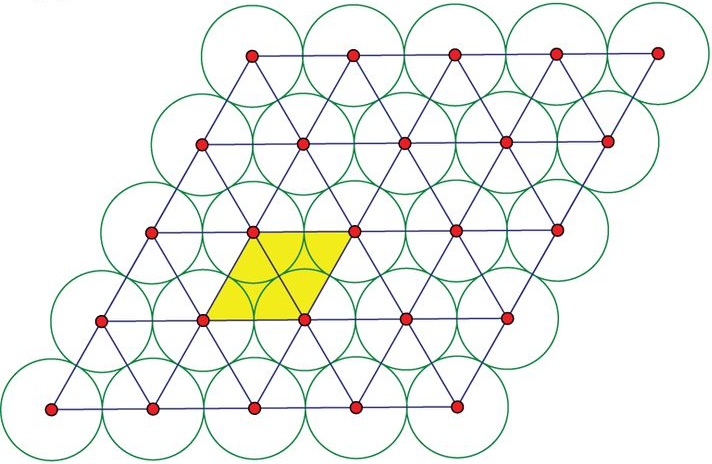
\includegraphics[width=0.5\linewidth]{./lect26/1.png}
\end{center}
Area of each disk is 
$$A(D) = \pi R^2$$
and area of ``triangle'' is
$$A(T) = \left(\sqrt{3} - \frac{\pi}{2}\right)R^2$$
Total covered area is
$$\frac{A(D)}{A(D) + 2A(T)} = \frac{\pi}{\sqrt{3} - \frac{\pi}{2}} \approx 0.907$$
Thus choosing random packing (two coordinates of center of one disk), probability of point to be not covered is
$$P(x_i) \approx 0.093$$
Then probability that at least one point is uncovered
$$P\left(\left\{ x_n\right\}  \right) \leq 10 \cdot P(x_i) = 10 \cdot 0.093 = 0.93 < 1$$
i.e. exist packing for which all 10 are covered.

\subsection{Secretary problem}
 In this game Alice, the informed player, writes secretly distinct numbers on $n$ cards. Bob, the stopping player, observes the actual values and can stop turning cards whenever he wants, winning if the last card turned has the overall maximal number.
 
 
Call strategy $j$ (for $j>0$) - to skip first $j$ numbers and then choose the first number bigger then all previous numbers. Denote by $W$ event of winning. What is $P_j(W)$ - probability to win using strategy $j$.
Denote by $A_k$ event that $k^{th}$ number is biggest.
$$P_j(A_k) = \frac{1}{n}$$
Find probability of winning via full probability
$$P_j(W) = \sum_{k=1}^n P(A_k)P(W|A_k) = \frac{1}{n} \sum_{k=1}^n P_j(W|A_k)$$
Now, if $1\leq k \leq j$,
$$P_j(W|A_k) = 0 $$
In other case, if maximum of first $k-1$ numbers is in first $j$ numbers, we win, else we lose, i.e.
$$P_j(W|A_k)  = \frac{j}{k-1}$$
Back to probability
$$P_j(W) =  \frac{1}{n} \sum_{k=j+1}^n \frac{j}{k-1}$$
Now lets perform asymptotic analysis for $j = \left[xn\right]$, $0<x<1$:

$$ \sum_{k=[xn]+1}^n \frac{1}{k-1} = \sum_{k=2}^n \frac{1}{k-1} - \sum_{k=2}^{[xn]} \frac{1}{k-1} \approx \log n - \log xn = -\log x$$
Thus
$$P_j(W) \approx -\frac{[xn]}{n} \log x = -x \log x$$
To maximize probability:
$$P'_j(W) = \log x + 1$$
$$\log x = -1$$
$$x = \frac{1}{e} \approx 0.368$$
And probability to win is 
$$P_j(W)  = -e^{-1} \log e^{-1} = e^{-1}\approx 0.368$$
\end{document}
